%% 
%% Copyright 2007-2020 Elsevier Ltd
%% 
%% This file is part of the 'Elsarticle Bundle'.
%% ---------------------------------------------
%% 
%% It may be distributed under the conditions of the LaTeX Project Public
%% License, either version 1.2 of this license or (at your option) any
%% later version.  The latest version of this license is in
%%    http://www.latex-project.org/lppl.txt
%% and version 1.2 or later is part of all distributions of LaTeX
%% version 1999/12/01 or later.
%% 
%% The list of all files belonging to the 'Elsarticle Bundle' is
%% given in the file `manifest.txt'.
%% 

%% Template article for Elsevier's document class `elsarticle'
%% with numbered style bibliographic references
%% SP 2008/03/01
%%
%% 
%%
%% $Id: elsarticle-template-num.tex 190 2020-11-23 11:12:32Z rishi $
%%
%%
\documentclass[preprint,12pt]{elsarticle}
\usepackage{orcidlink}
\hypersetup{hidelinks}
\usepackage{adjustbox}
\usepackage{rotating}
\usepackage[caption=false, font=footnotesize]{subfig}

\newcommand*\sumta[2]{\mathop {\sum} \limits_{#1}^{#2}}
%% Use the option review to obtain double line spacing
%% \documentclass[authoryear,preprint,review,12pt]{elsarticle}

%% Use the options 1p,twocolumn; 3p; 3p,twocolumn; 5p; or 5p,twocolumn
%% for a journal layout:
%% \documentclass[final,1p,times]{elsarticle}
%% \documentclass[final,1p,times,twocolumn]{elsarticle}
%% \documentclass[final,3p,times]{elsarticle}
%% \documentclass[final,3p,times,twocolumn]{elsarticle}
%% \documentclass[final,5p,times]{elsarticle}
%% \documentclass[final,5p,times,twocolumn]{elsarticle}

%% For including figures, graphicx.sty has been loaded in
%% elsarticle.cls. If you prefer to use the old commands
%% please give \usepackage{epsfig}

%% The amssymb package provides various useful mathematical symbols
\usepackage{amssymb}
\usepackage{booktabs}
\usepackage[utf8]{inputenc}
\usepackage{amsmath} % For math symbols like \sum, \sqrt, \bar
\usepackage{array}
\usepackage{graphicx}

\usepackage{multirow}

%% The amsthm package provides extended theorem environments
%% \usepackage{amsthm}

%% The lineno packages adds line numbers. Start line numbering with
%% \begin{linenumbers}, end it with \end{linenumbers}. Or switch it on
%% for the whole article with \linenumbers.
%% \usepackage{lineno}

\journal{Decision Analytics Journal}

\begin{document}

\begin{frontmatter}

%% Title, authors and addresses

%% use the tnoteref command within \title for footnotes;
%% use the tnotetext command for theassociated footnote;
%% use the fnref command within \author or \address for footnotes;
%% use the fntext command for theassociated footnote;
%% use the corref command within \author for corresponding author footnotes;
%% use the cortext command for theassociated footnote;
%% use the ead command for the email address,
%% and the form \ead[url] for the home page:
%% \title{XAI-Based Sensor Selection Framework for Finger Position Recognition}
%% \tnotetext[label1]{}
%% \author{Name\corref{cor1}\fnref{label2}}
%% \ead{email address}
%% \ead[url]{home page}
%% \fntext[label2]{}
%% \cortext[cor1]{}
%% \affiliation{organization={},
%%             addressline={},
%%             city={},
%%             postcode={},
%%             state={},
%%             country={}}
%% \fntext[label3]{}

\title{Physiologically Interpretable Machine Learning Framework for Electromyography Sensor Optimization in Finger Movement Recognition}

%% use optional labels to link authors explicitly to addresses:
%% \author[label1,label2]{}
%% \affiliation[label1]{organization={},
%%             addressline={},
%%             city={},
%%             postcode={},
%%             state={},
%%             country={}}
%%
%% \affiliation[label2]{organization={},
%%             addressline={},
%%             city={},
%%             postcode={},
%%             state={},
%%             country={}}

\author[inst1]{Minh-Tri Ta\orcidlink{0009-0002-4570-6114}}
% \corref{contrib}
\author[inst2, inst3]{Hoang-Khang Phan\orcidlink{0009-0007-1578-0977}}
% \corref{contrib}
\author[inst4, *]{Le-Giang Tran\orcidlink{0000-0003-4458-6229}}

\affiliation[inst1]{organization={... VinUniversity}, city={Ho Chi Minh City}, country={Vietnam}}           
\affiliation[inst2]{organization={Department of Biomedical Engineering, Faculty of Applied Science, Ho Chi Minh City University of Technology (HCMUT)}, addressline={268 Ly Thuong Kiet Street, District 10}, city={Ho Chi Minh City}, country={Vietnam}}
\affiliation[inst3]{organization={Vietnam National University Ho Chi Minh City}, addressline={Linh Trung Ward, Thu Duc City}, city={Ho Chi Minh City}, country={Vietnam}}
\affiliation[inst4]{organization={Faculty of Electronics Technology, Industrial University of Ho Chi Minh City}, city={Ho Chi Minh City}, country={Vietnam}}
\affiliation[*]{Corresponding author: tranlegiang@iuh.edu.vn}

%\ead{tranlegiang@iuh.edu.vn}
% % PUBLIC CODE BASE IF NEEDED
% \cortext[code]{Code repository:}
\begin{abstract}
%% Text of abstract
Accurate recognition of finger position and movement remains a challenging problem for various applications, including human-computer interaction, virtual reality, and prosthetic control. Current surface electromyography (sEMG)-based finger recognition systems often rely on increasing the density of the sensor array and computational power. Meanwhile, existing sensor selection methods rarely provide physiologically interpretable evidence on sensor importance. To address this issue, this work proposed a physiologically interpretable, explainable artificial intelligence (xAI) sensor selection framework that enables us to precisely optimize the number of sEMG sensors for finger position classification systems. We evaluated the framework on four machine and deep learning models, namely XGBoost, Random Forest, Support Vector Machine (SVM), and Convolutional Neural Network (CNN), on the NinaPro DB5 dataset. Results indicated that XGBoost and Random Forest exhibited higher performance among other models in finger position classification, achieving an accuracy of approximately 84\% in random splits and approximately 71\% in leave-one-subject-out (LOSO) cross-validation. Then, Feature importance derived from the explainable models was subsequently interpreted with forearm muscle physiology to identify the most significant sEMG channels for finger movement recognition.
Finally, the top five sEMG channels that outperformed the full channels configuration with an accuracy of 84\% and a weighted F1 score of 80\% were identified. These results demonstrated that xAI was able to identify physiologically meaningful muscle activation patterns, enabling efficient sensor reduction without compromising accuracy, and ultimately improving clinical applicability.
\end{abstract}



\begin{keyword}
%% keywords here, in the form: keyword \sep keyword
Machine learning \sep sensor optimization \sep  explainable AI \sep  feature analysis \sep classification accuracy \sep interpretable models.
% PACS codes here, in the form: \PACS code \sep code
% \PACS 0000 \sep 1111
% %% MSC codes here, in the form: \MSC code \sep code
% %% or \MSC[2008] code \sep code (2000 is the default)
% \MSC 0000 \sep 1111
\end{keyword}

\end{frontmatter}

%% \linenumbers

%% main text

\section{Introduction}
Accurate recognition of finger positions and movements is an important requirement in myoelectric prosthesis control, rehabilitation robotics, human–computer interaction, and virtual and augmented reality systems. Surface electromyography (sEMG) is particularly suitable for these applications because it provides a non-invasive means of measuring the electrical activity associated with voluntary muscle activation. By extracting movement-related information from forearm sEMG signals, computational models can translate neuromuscular activity into commands for external devices. Nevertheless, reliable recognition of individual finger movements remains challenging because finger control involves multiple degrees of freedom, overlapping muscle functions, and substantial variability in the recorded sEMG patterns.

%The loss of an upper limb is a profound event that reverberates through an individual's life, impacting physical function, psychological well-being, and overall quality of life. This can manifest in several ways, including difficulty performing activities of daily living (ADLs) such as dressing, eating, and grooming \cite{1}. Amputation can also lead to social isolation, depression, and anxiety as individuals grapple with the physical and emotional challenges of their new reality \cite{2}. Furthermore, the loss of limb function can significantly impact a person's sense of self-identity and body image \cite{3}. However, the advent of surface electromyography (sEMG) controlled prosthetic hands has ignited a spark of hope, offering a potential avenue for restoring autonomy and facilitating reintegration into daily life \cite{2}. These innovative devices decode the subtle electrical signals generated by residual muscles, translating them into commands for prosthetic hand movement.

However, despite of the advancement of sEMG signal decoding in machine learning (ML) and deep learning (DL) algorithms, their "black box" nature poses a significant barrier to widespread clinical adoption and user trust \cite{4} The lack of transparency in these complex models hinders understanding of their decision-making processes, raising concerns about their reliability and safety, particularly in real-world scenarios with unpredictable challenges \cite{5}. To mitigate these 'black box' problems, Explainable Artificial Intelligence (XAI) provides methodologies for enhancing model transparency and interpretability. The critical role of these advancements for trustworthy decision analytics was often highlighted in comprehensive reviews that map recent developments and future trends within the XAI field\cite{saranya2023systematic}. XAI also emerges as a beacon of clarity in this landscape, offering a promising solution to unravel the complexities of sEMG signal decoding \cite{6}. By providing interpretable explanations for model predictions, highlighting salient features, and visualizing decision pathways, XAI methods like Local Interpretable Model-Agnostic Explanations (LIME) \cite{7}, Shapley Additive Explanations (SHAP) \cite{8}, and Layer-wise Relevance Propagation (LRP) \cite{9} shed light on the mechanisms governing prosthetic hand control.

Incorporating XAI into sEMG-controlled prosthetic hands not only enhances their transparency and trustworthiness but also paves the way for continuous refinement and personalization \cite{10}. By deciphering the intricate relationship between muscle signals and intended movements, researchers and clinicians can identify potential sources of error, optimize control algorithms, and tailor prosthetic hand function to individual needs \cite{11}. This personalized approach can lead to more intuitive and natural control, enhancing user satisfaction and facilitating seamless integration into daily life \cite{12}. XAI marks a turning point in prosthetic technology, empowering users to grasp their rehabilitation journey. With every controlled movement, users of XAI-enhanced prosthetics reclaim independence, redefine their potential, and usher in a future where human resilience and technological brilliance overcome limitations. This powerful fusion of human spirit and advanced technology promises a more inclusive future, where individuals with limb differences can live life to the fullest.

\section{Background and Related works}
The pursuit of creating a robotic hand capable of autonomous object manipulation, as envisioned by Cutkosky in 1989 \cite{13}, has spurred extensive research in the field of rehabilitation robotics. Central to this endeavor is the development of sEMG-controlled prosthetic hands, which aim to empower amputees by restoring lost motor function. While sEMG-based approaches have shown promise, their clinical translation and user acceptance have been hampered by the complexity of sEMG signals and the limitations of traditional machine learning (ML) models.

Early research in sEMG-controlled prosthetic hands focused on developing pattern recognition algorithms to decode hand movements from sEMG signals \cite{13,14}. However, achieving consistently high classification accuracies across a wide range of movements proved challenging, with results often reach from 70 to over 90\% \cite{15,Zhouping,s20030672,16,17,18}. This limitation is partly attributed to the inherent variability of sEMG signals, which are influenced by individual differences, muscle fatigue, and electrode placement and quality.

Particularly, Palermo et al. \cite{16} investigated the repeatability of grasp recognition using sEMG and a Random Forest model, achieving an average accuracy of 50\%, with a peak accuracy of 82\%. However, they also observed a decrease in accuracy between morning and afternoon tests, suggesting diurnal variations in sEMG signals and finger posture. Ding et al.\cite{17} explored the use of convolutional neural networks (CNNs) for hand posture recognition, utilizing 12 electrodes and a combination of traditional ML and deep learning algorithms. They achieved average accuracies of 78\% and 84\%, respectively, highlighting the potential of deep learning for sEMG signal decoding. Zhang et al.\cite{18} further demonstrated the effectiveness of classical ML methods, employing various techniques and features such as MAV, WL, ZC, and slope sign change. Their research achieved model accuracies ranging from 77\% to 93\% across 17 activity categories in the Ninapro dataset. In addition to that, Zhang and his colleagues also tested the method on their dataset, cross-validating that their proposed framework can achieve accuracy up to 93\% in hand posture recognition.

However, most research relies on user-dependent methods, which introduce significant bias into experimental results and hinder real-world deployment \cite{13,14,15,Zhouping,17,18}. For instance, Chen et al. \cite{s20030672} observed a substantial accuracy drop to 69\% in their finger gesture recognition experiments using a random train-valid-test framework. This highlights the critical need for robust, cross-person frameworks, especially a comprehensive user-independent framework for finger movement recognition.

Surface electromyography does not directly measure individual muscle force or joint motion. Instead, an sEMG channel records the volume-conducted summation of motor-unit action potentials generated by active muscle fibers within the detection volume of the electrode. The resulting signal is therefore affected by motor-unit recruitment and discharge behavior, muscle-fiber geometry, electrode location and orientation, subcutaneous tissue, and contributions from adjacent muscles. Consequently, the information captured by sEMG reflects both the neural activation associated with the intended movement and the biomechanical properties of the hand \cite{s21217322, alcan2023current}. 

Recent developments in sEMG analysis have accordingly emphasized the interpretation of spatial activation patterns, muscle coordination, and motor synergies in addition to conventional classification performance \cite{s21217322}. These studies, employing various ML and DL techniques, have achieved a range of performance outcomes and highlighted persistent challenges, particularly in user-independent scenarios and system optimization. Addressing these challenges in system optimization and achieving high performance often involves sophisticated model tuning and feature engineering. Recent work demonstrated the application of hybrid deep neural network models combined with optimization techniques like randomized search, cross-validation, and feature selection to enhance predictive accuracy in areas such as coronary heart disease prediction \cite{sharma2023hybrid}. To provide a structured overview and better contextualize the contributions of the present study against this backdrop, Table \ref{tab:related_works_comparison} summarizes key aspects of these pertinent related works alongside the approach and findings of our research. This comparative summary aims to delineate the specific advancements offered by our XAI-integrated framework.

Existing methods for classifying hand movements using sEMG signals often exhibit limitations such as restricted accuracy, inconsistent performance, a reliance on a high number of sensors, and a lack of cross-subject validation. To address these gaps, this study aims to develop ML and DL pipelines for user-independent sEMG signal classification of hand movements. XAI techniques, specifically SHAP and Grad-CAM, will be implemented to interpret SVM, ANN, and CNN models. The primary contributions of this research are: (1) The development and validation of a novel XAI-integrated sensor selection framework designed to optimize the number of sEMG channels required for real-time prosthetic hand applications, thereby enhancing system efficiency and potential user comfort while maintaining high classification accuracy; (2) The demonstration of data-driven optimization of sEMG features, achieved through the integration of XAI results and physiology insights. In the present framework, physiological interpretation is used as an external plausibility criterion for the XAI results rather than as a direct anatomical identification of each recorded channel.

\newcolumntype{L}[1]{>{\raggedright\arraybackslash}p{#1}}
\newcolumntype{C}[1]{>{\centering\arraybackslash}p{#1}} % Centered wrapped column
\begin{sidewaystable}[!htbp]
\centering\
\caption{Comparison of current works in sEMG-based Hand/finger movement recognition}
\label{tab:related_works_comparison}
\large
\resizebox{\textwidth}{!}{%
\begin{tabular}{L{4cm} L{3.5cm} C{1.5cm} L{3cm} L{2.5cm} L{7cm} L{7cm}}
\toprule
\textbf{Study (Citation)} & \textbf{Task / Dataset Focus} & \textbf{No. of Electrodes} & \textbf{Key Method(s)} & \textbf{Validation Scheme} & \textbf{Reported Performance Metric(s)} & \textbf{Relevance / Comparison to Current Work} \\
\midrule

General Early Research \cite{13,14,15,Zhouping,16,17,18} & sEMG pattern recognition for hand movements & Varied & Pattern Recognition Algorithms & Often User-Dependent & Accuracies: 70\% to $>$ 90\% & Established the field; highlighted challenges in achieving consistent high accuracy and robustness. \\
\addlinespace

Palermo et al. (2017) \cite{16} & Grasp recognition (NinaPro DB5 subset) & Varied (Full Ninapro setup) & sEMG, Random Forest & User-dependent split (50/50) & Avg. Accuracy: $\sim 50\%$, Peak: $82\%$ & Investigated repeatability; showed diurnal variations. focused on specific finger positions rather than grasps. \\
\addlinespace

Ding et al. (2018) \cite{17} & Hand posture recognition (sEMG) & 12 & CNNs, Traditional ML & User-dependent & Avg. Accuracies: CNN: $84\%$, Trad. ML: $78\%$ & Demonstrated potential of deep learning used CNN and incorporates XAI for sensor optimization. \\
\addlinespace

Zhang et al. (2024) \cite{18}  & Hand gesture/activity recognition (Ninapro DB5 - 17 activities; also custom dataset) & Varied & Classical ML (MAV, WL, ZC, slope sign change), Sliding Voting Classifiers & (Not specified, user-dependent mentioned as general issue) & Accuracy: $77\%$ to $93\%$ (Ninapro); Up to $93\%$ (custom) & Showed effectiveness of classical ML. Current work uses some similar models but focuses on 13 finger positions and XAI-driven sensor reduction. \\
\addlinespace

Chen et al. (2017) \cite{s20030672} & Finger gesture recognition (sEMG) & Not specified & Compact ENN & Random train-valid-test & Accuracy drop to $69\%$ & Highlighted significant accuracy drop in less user-dependent setups, motivating robust interpersonal frameworks. \\
\addlinespace
\hline
\addlinespace
\textbf{This Work} & \textbf{13 Finger Positions (NinaPro DB5)} & \textbf{16 sEMG (optimized to 5-10)} & \textbf{Time-domain features; ML (XGB, RF, SVM), CNN; XAI (SHAP, Grad-CAM) for sensor selection} & \textbf{Random Split (70/30), Interpersonal Cross-validation (LOSO)} & \textbf{Random (16 sens): Acc $\sim 84-85\%$ (XGB,RF,CNN). LOSO (16 sens): Acc $\sim 71\%$ (XGB,RF,SVM). Optimized (5-10 sens, random): Acc $\sim 84\%$, F1 $\sim 80\%$} & \textbf{Develops an XAI-integrated framework for user-independent finger position recognition, optimizing sensor quantity while maintaining high accuracy and providing model interpretability.} \\
\bottomrule
\end{tabular}%
}
\vspace{2mm}
\end{sidewaystable}
% VERTICAL_TABLE_____________________________
% \begin{table}[!htbp] % Using !htbp for better float placement
% \centering
% \caption{Comparison of current works in sEMG-based Hand/Finger Movement Recognition}
% \label{tab:related_works_comparison}
% \resizebox{\textwidth}{!}{% Use \resizebox to fit table to text width; adjust if needed
% \begin{tabular}{L{2.5cm} L{3.5cm} C{1.5cm} L{3cm} L{2.5cm} L{3cm} L{4cm}}
% \toprule
% \textbf{Study (Citation)} & \textbf{Task / Dataset Focus} & \textbf{No. of Electrodes} & \textbf{Key Method(s)} & \textbf{Validation Scheme} & \textbf{Reported Performance Metric(s)} & \textbf{Relevance / Comparison to Current Work} \\
% \midrule

% General Early Research \cite{13,14,15,Zhouping,16,17,18} & sEMG pattern recognition for hand movements & Varied & Pattern Recognition Algorithms & Often User-Dependent & Accuracies: 70\% to $>$ 90\% & Established the field; highlighted challenges in achieving consistent high accuracy and robustness. \\
% \addlinespace

% Palermo et al. (2017) \cite{16} & Grasp recognition (NinaPro DB5 subset) & Varied (Full Ninapro setup) & sEMG, Random Forest & (Not specified) & Avg. Accuracy: $\sim 50\%$, Peak: $82\%$ & Investigated repeatability; showed diurnal variations. Current work focuses on specific finger positions rather than grasps. \\
% \addlinespace

% Ding et al. (2018) \cite{17} & Hand posture recognition (sEMG) & 12 & CNNs, Traditional ML & (Not specified) & Avg. Accuracies: CNN: $84\%$, Trad. ML: $78\%$ & Demonstrated potential of deep learning. Current work also uses CNN but incorporates XAI for sensor optimization. \\
% \addlinespace

% Zhang et al. (2024) \cite{18}  & Hand gesture/activity recognition (Ninapro DB5 - 17 activities; also custom dataset) & Varied & Classical ML (MAV, WL, ZC, slope sign change), Sliding Voting Classifiers & (Not specified, user-dependent mentioned as general issue) & Accuracy: $77\%$ to $93\%$ (Ninapro); Up to $93\%$ (custom) & Showed effectiveness of classical ML. Current work uses some similar models but focuses on 13 finger positions and XAI-driven sensor reduction. \\
% \addlinespace

% Chen et al. (2017) \cite{s20030672} & Finger gesture recognition (sEMG) & Not specified & Compact ENN & Random train-valid-test & Accuracy drop to $69\%$ & Highlighted significant accuracy drop in less user-dependent setups, motivating robust interpersonal frameworks . \\
% \addlinespace
% \hline
% \textbf{Our Work} & \textbf{13 Finger Positions (NinaPro DB5)} & \textbf{16 sEMG (optimized to 5-10)} & \textbf{Time-domain features; ML (XGB, RF, SVM), CNN; XAI (SHAP, Grad-CAM) for sensor selection} & \textbf{Random Split (70/30), Interpersonal Cross-validation (LOSO)} & \textbf{Random (16 sens): Acc $\sim 84-85\%$ (XGB,RF,CNN). LOSO (16 sens): Acc $\sim 71\%$ (XGB,RF,SVM). Optimized (5-10 sens, random): Acc $\sim 84\%$, F1 $\sim 80\%$} & \textbf{Develops an XAI-integrated framework for user-independent finger position recognition, optimizing sensor quantity while maintaining high accuracy and providing model interpretability.} \\
% \bottomrule
% \end{tabular}%
% }
% \vspace{2mm}

% \end{table}

%\begin{enumerate}

%\item \textbf{Objective 1}: Propose the novel XAI-integrated ML pipeline for user independent sEMG signal decoding. Investigation in the integration of various XAI techniques, including SHAP, and GRAD-CAM, with different traditional ML models, and DL models, including SVM, ANN, and CNNs, to enhance their interpretability and performance in sEMG signal classification.
   % \item \textbf{Objective 2}: Quantify the impact of XAI in propose pipeline: We will assess the improvement in accuracy, precision, recall, and F1-score of XAI-enhanced models compared to traditional ML models using the NinaPro DB5 dataset.
   % \item In current search, the number of sEMG sensors often lays between 8 to 16 sensors\cite{15,16,17,18}. \textbf{(RQ1)} Is that number of sensors is optimal for prosthetic hand applications? If that not optimal for the task, can we lower the number of sensor needed? 
   % \item Given that XAI is capable of understanding the contribution of features in the model decision. \textbf{(RQ2)} /Can XAI highlight the factor that driven the model to its decision?  
%\end{enumerate}

\section{Methodology}

\begin{figure}[!ht]
    \centering
    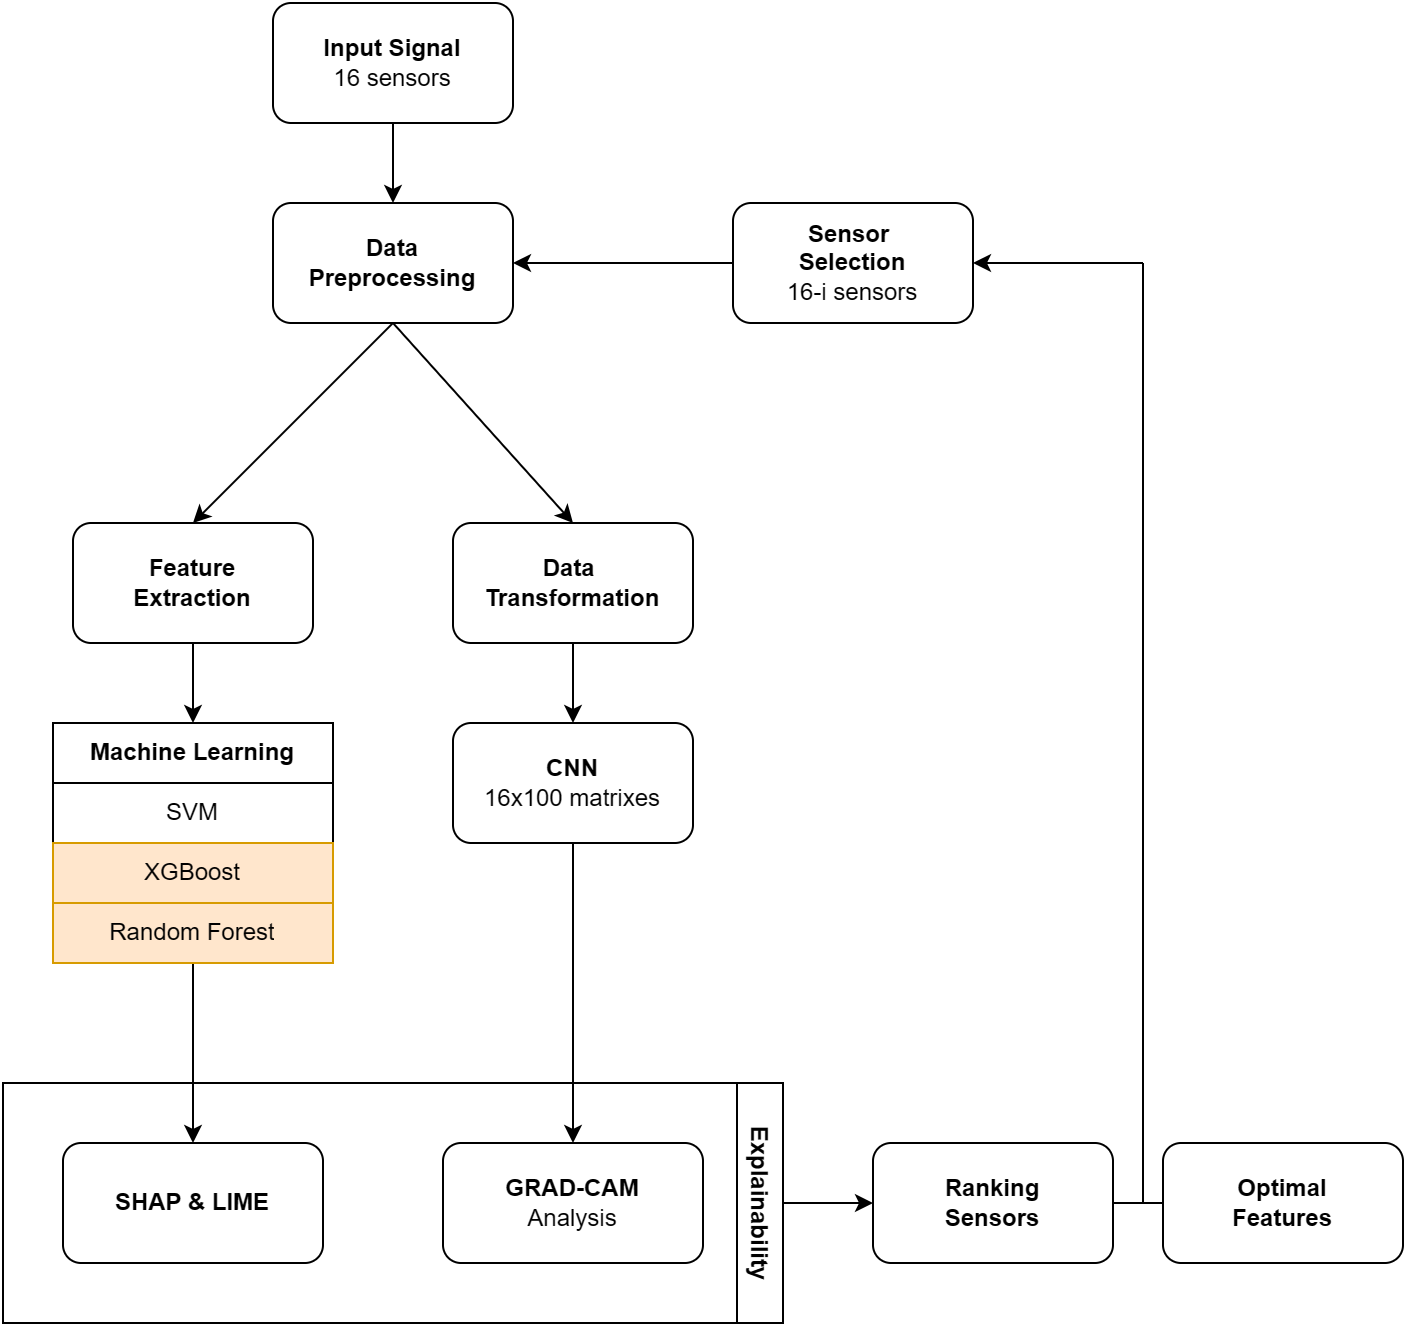
\includegraphics[width=0.75\linewidth]{Figure_1_The block diagram of XAI-based classification model.png}
    \caption{The block diagram of XAI-based classification model}
    \label{method_fc}
\end{figure}

This study delineates a rigorous methodology employed to investigate the real-time control and detection of hand movements utilizing sEMG sensors bolstered by XAI tools. The methodology encompasses several key components, including a comprehensive understanding of the NinaPro dataset, preprocessing steps involving various filtering and signal processing techniques tailored to sEMG data, exploration and selection of optimal feature extraction methods specific to the problem domain, integration of XAI algorithms alongside classification models for effective gesture classification, and thorough evaluation utilizing a range of performance metrics. The processing will be followed by the pipeline in Figure \ref{method_fc}.

\subsection{Dataset}

The DB5 dataset from the NinaPro repository was utilized for feature extraction and insight analysis in this work \cite{19}. It includes recordings from 10 subjects performing 52 unique hand movements, providing comprehensive data for model development and evaluation. Each movement is recorded using a multi-sensor setup that captures various modalities, including sEMG, kinematic data, and inertial information. 

\begin{table}[!htbp]
\centering
\caption{Detailed characteristics of the NinaPro DB5 dataset subset and subject demographics used}

\label{tab:dataset_subject_details}
\begin{tabular}{L{5cm} L{7cm}} 
\toprule
\textbf{Characteristic} & \textbf{Value / Details} \\
\midrule
\textbf{Dataset Source} & NinaPro (Non-Invasive Adaptive Prosthetics) Project - Database 5 (DB5) \\
\addlinespace
\textbf{Number of Subjects Utilized} & 10 \\
\addlinespace
\textbf{Age of Subjects (Mean $\pm$ SD)} & $34.9 \pm 11.8$ years \\
% Consider adding Range if available and relevant, e.g., (Range: XX - YY years)
\addlinespace
\textbf{Gender Distribution} & 8 Male, 2 Female  \\
\addlinespace
\textbf{Handedness} & 10 Right \\
\addlinespace
\textbf{Movements Profile} & \\
\textit{Total in DB5} & 52 unique hand movements \\
\textit{Selected for this study} & 13 finger positions (12 finger gestures + 1 resting state, extracted from the 52 movements) \\
\textit{Repetitions per Movement} & 6  \\
\addlinespace
\textbf{sEMG Acquisition Setup} & \\
\textit{Electrodes Used} & 16 active differential sEMG electrodes \\
\textit{Device(s)} & Two Thalmic Myo armbands (each with 8 electrodes) \\
\textit{Electrode Configuration/Placement} & As per NinaPro DB5 standard protocol (e.g., equally spaced around the forearm at a specific location) \\
\textit{Sampling Rate} & 200 Hz  \\
\bottomrule
\end{tabular}
\vspace{2mm}
\end{table}


The dataset comprises sEMG signals from 16 electrodes using two Thalmic Myo armbands and all information on the age and sex of the subjects, body size, handedness, and forearm circumference of subjects (see Table \ref{tab:dataset_subject_details}). The datasets are widely available to be used from the NinaPro\footnote{https://ninapro.hevs.ch/instructions/DB5.html} website, together with the detailed documentation herein guiding exploration \cite{20}.
In this work, 13 finger positions, including 12 finger gestures and 1 resting state, were extracted from 52 hand movements \cite{19} to obtain an analysis regarding their contribution with every movements (Figure \ref{12_movement}). All subjects of these datasets will be used to assess the performance of XAI algorithms and find similarities in the hand movement patterns. By focusing learning on just these finger positions, it is hoped to allow a more granular comparison amongst sensor contributions and give insight into the subtleties of hand movement analysis.

\begin{figure}[!ht]
    \centering
    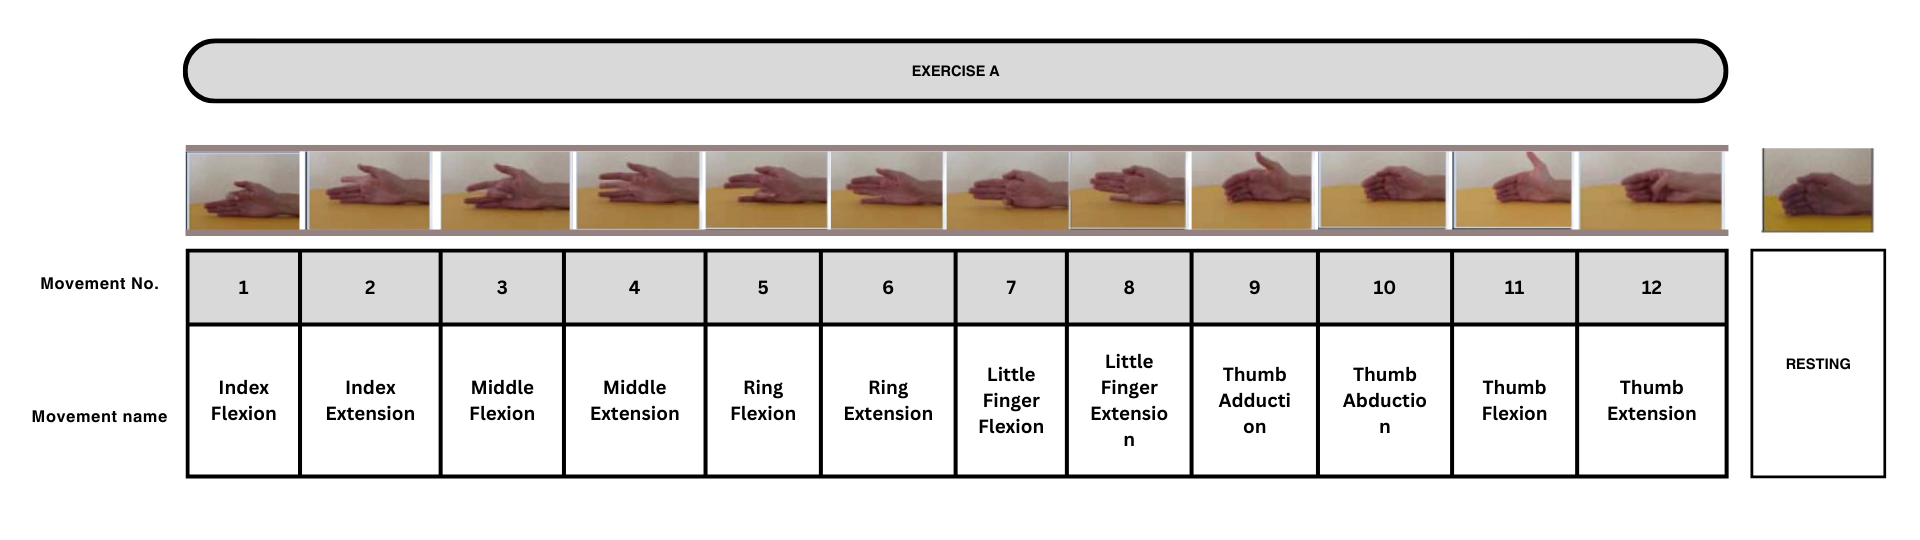
\includegraphics[width=1\linewidth]{Figure_2_12classesofDB5.png}
    \caption{Finger and Thumb Movement Classes in the NinaPro DB5 Dataset}
    \label{12_movement}
\end{figure}

\subsection{Feature extraction}
In this work, 16 sensors from the dataset were treated differently in machine learning and deep learning approaches. 
In  ML approach, we extracted a total of 8 statistical features, namely min, max, median, mean, skew, IQR, RMS, and entropy (see table \ref{tab:features_definition_full}) from each sensor data with a window size of 500 ms with an overlap rate of 0 ms via tsfel services \cite{tsfel}. In previous works, time-domain features were proved to be effective in finger position recognition via sEMG data \cite{15,stat_sEMG,18}.


\begin{table}[!ht]
    \centering
    \caption{Definition of Selected Time-Domain Features}
    \label{tab:features_definition_full} % Changed label for clarity
    % \vspace{10px} % This vspace might be better outside the resizebox or removed if booktabs spacing is sufficient
    
    \resizebox{\textwidth}{!}{% Add \resizebox here
    \begin{tabular}{l l L{6cm}} % Adjusted the width in L{} slightly for the example, you might need to fine-tune
    \toprule % Using booktabs style, or replace with \hline
        \textbf{Feature Name} & \textbf{Formula} & \textbf{Definition} \\
    \midrule % Using booktabs style, or replace with \hline
        Minimum (Min) & $min(x_1, ..., x_n)$ & The smallest amplitude value in the sEMG signal segment, indicating the lowest level of muscle activity recorded. \\
    \addlinespace % Adds a little space between rows, good with booktabs
        Maximum (Max) & $max(x_1, ..., x_n)$ & The largest amplitude value in the sEMG signal segment, representing the peak muscle activity recorded. \\
    \addlinespace
        Median & $median(x_1, ..., x_n)$ & The middle value of the sEMG signal amplitudes in a segment when sorted, providing a measure of central tendency robust to outliers. \\
    \addlinespace
        Mean & $\bar{x} = \frac{1}{n}\sum_{i=1}^{n}x_i$ & The average amplitude of the sEMG signal in a segment, reflecting the overall level of muscle contraction. \\
    \addlinespace
        Skewness & $ \frac{\frac{1}{n}\sum_{i=1}^{n}(x_i - \bar{x})^3}{(\frac{1}{n}\sum_{i=1}^{n}(x_i - \bar{x})^2)^{3/2}} $ & A measure of the asymmetry of the probability distribution of sEMG signal amplitudes around its mean. \\
    \addlinespace
        Interquartile Range (IQR) & $Q_3 - Q_1$ & The range between the first quartile ($Q_1$) and the third quartile ($Q_3$) of sEMG signal amplitudes, representing the spread of the middle 50\% of the data. \\
    \addlinespace
        Root Mean Square (RMS) & $ \sqrt{\frac{1}{n}\sum_{i=1}^{n}x_i^2} $ & A measure of the sEMG signal's power or intensity, reflecting the level of muscle activity over a segment. \\
    \addlinespace
        Entropy & $-\sum_{k}P(s_k)\log_2 P(s_k)$ & A measure of the complexity or irregularity of the sEMG signal, where $P(s_k)$ is the probability of the signal being in state $s_k$. \\
    \bottomrule % Using booktabs style, or replace with \hline
    \end{tabular}%
    } % Close \resizebox here
\end{table}

\subsection{Data transformation}

In the deep learning pipeline, the preparation of surface EMG data for CNN classification involved a structured sequence of preprocessing and transformation steps to ensure the data was both informative and suitable for the network's requirements.

First, the continuous sEMG signals were segmented into non-overlapping windows of 500 ms. This window length was selected to capture the temporal dependencies and dynamic patterns in muscle activity, which are critical for distinguishing between different movement classes. Each window was then inspected to verify dimensional correctness, ensuring consistency in the input format and preventing errors during CNN processing.

Following segmentation, standardization was performed on the sensor data within each window. This step involved scaling the data to have a zero mean and unit variance, thereby normalizing the features across all windows. Standardization was critical to mitigate the influence of variations in signal amplitude, ensuring that features with larger magnitudes did not dominate the learning process or introduce bias into the model.

After standardization, the processed sensor data for each window was transformed into a visual representation. Specifically, the standardized values were mapped to color intensities to generate a color image for each window, where the amplitude of the sEMG signals was reflected by the intensity and distribution of colors. This transformation allowed the CNN to leverage its ability to learn spatial patterns, treating the visualized sEMG data as image-like inputs.

These generated images were then organized and labeled according to their corresponding movement or class, creating a labeled dataset suitable for supervised learning. By representing the sEMG signals in this manner, the CNN was enabled to learn intricate spatial and temporal patterns within the data, thereby enhancing its ability to classify and predict different motor activities effectively.

\begin{table}[!htbp]
\centering
\caption{Summary of data preprocessing steps for machine learning and deep learning pipelines}
\label{tab:data_preprocessing_summary}
\resizebox{\textwidth}{!}{%
\begin{tabular}{L{3.5cm} L{3cm} L{3.5cm} L{3cm} L{4cm} L{3cm} L{4cm}}
\toprule
\textbf{Pipeline} & \textbf{Initial Input Signal} & \textbf{Segmentation / Windowing} & \textbf{Feature Engineering / Data Transformation} & \textbf{Normalization / Standardization} & \textbf{Final Input to Model} \\
\midrule
\textbf{ML Approach} & Raw sEMG data from 16 sensors & Window size: 500 ms; Overlap: 0 ms (non-overlapping) & Extraction of 8 time-domain features (Min, Max, Mean, etc. via tsfel) & Standard Scaler & Feature vectors (1 vector per window per sensor, or combined) \\
\addlinespace
\textbf{DL Approach (CNN)} & Raw sEMG data from 16 sensors & Window size: 500 ms (non-overlapping mentioned in Sec 3.3)  & Transformation of standardized windowed sEMG data into color images (16x100 matrix to image) & Standardization within each window (zero mean, unit variance) applied before image transformation & Labeled images (16x100 pixels, 3 channels if color) \\
\bottomrule
\end{tabular}%
}
\vspace{2mm}
\end{table}


\subsection{Classification model}
In this work, three machine learning models, namely Random Forest, Extreme Gradient Boosting, and Support Vector Machine, and one DL-based CNN model are being used to train and explain the importance of each factor that drives model decision.


\begin{figure}[!ht]
    \centering
    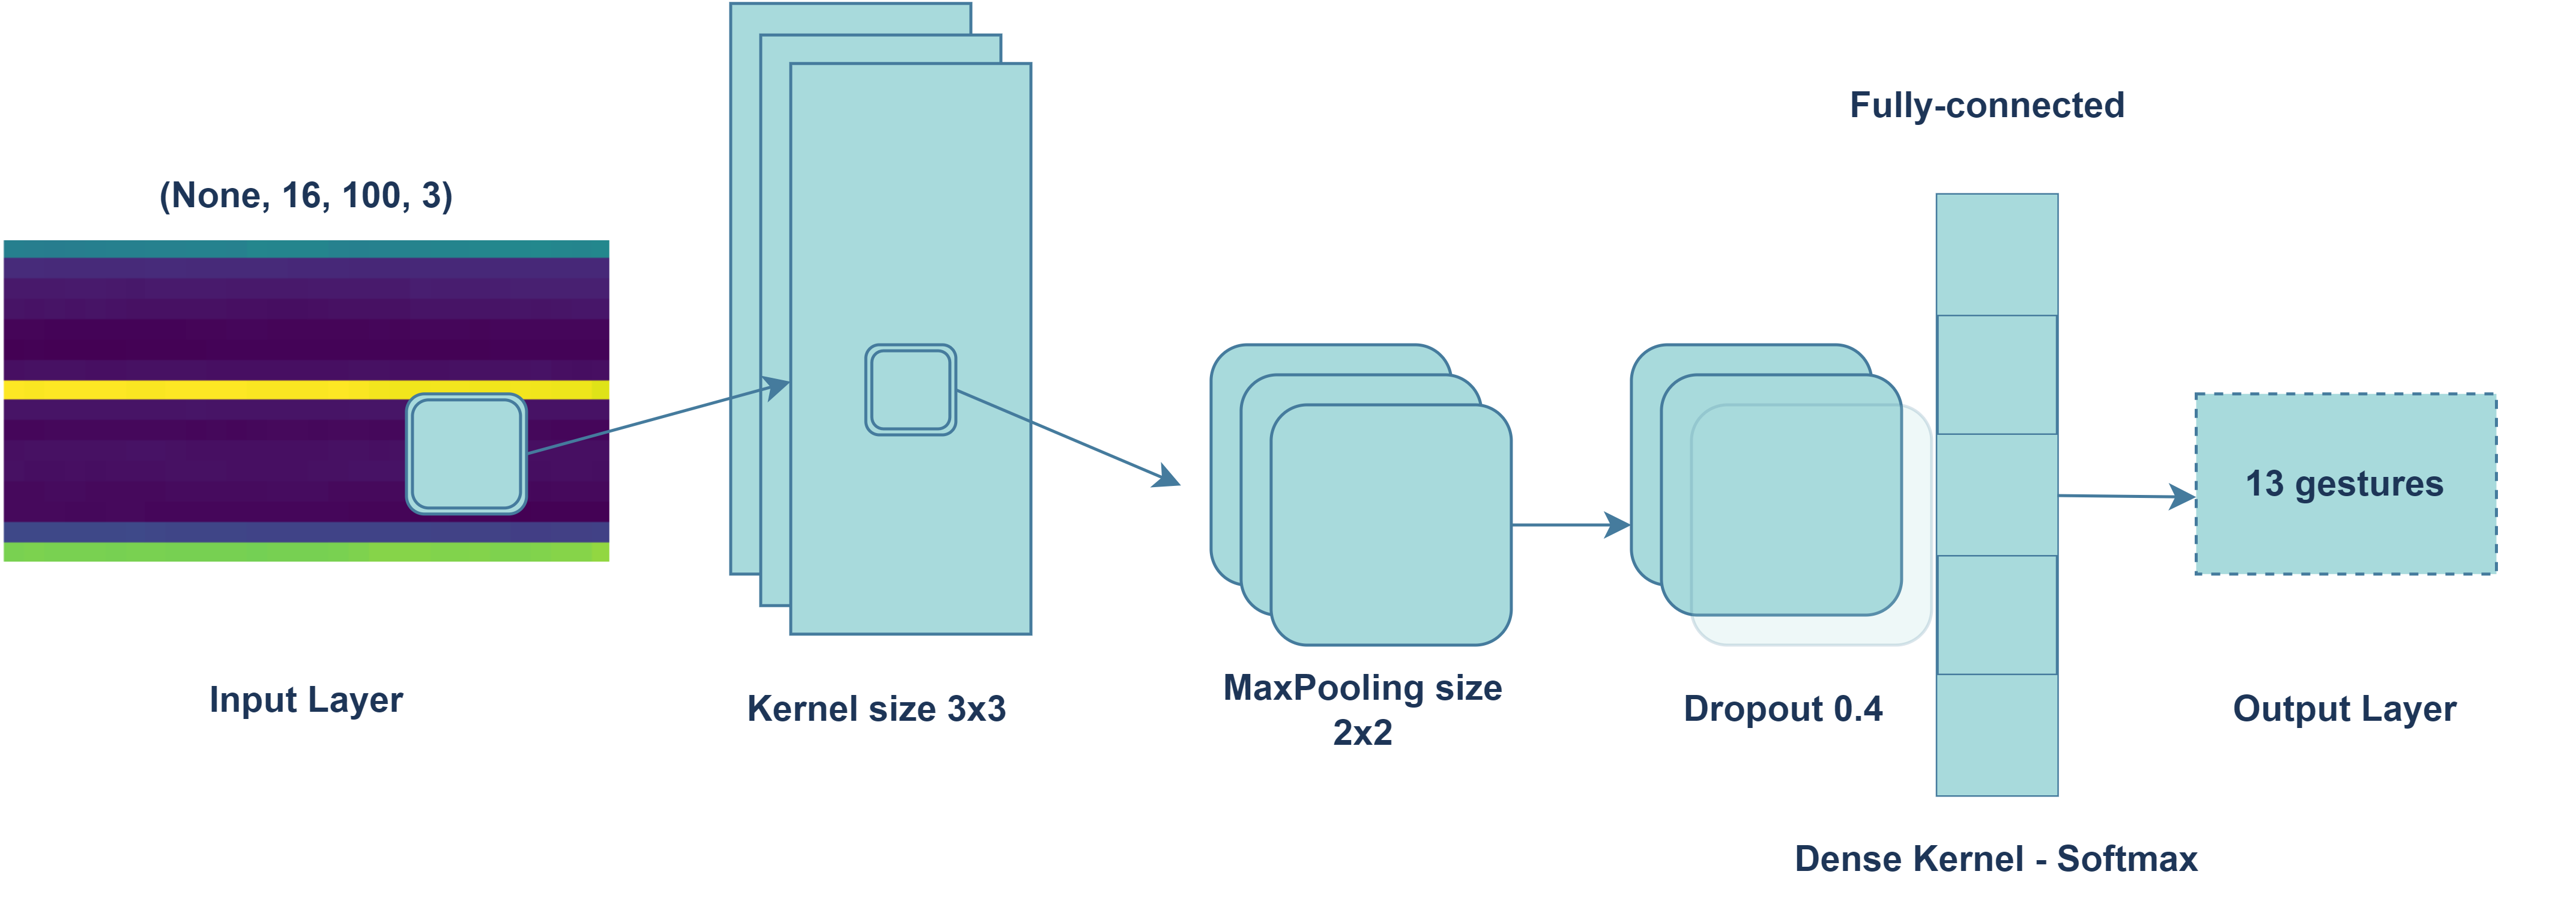
\includegraphics[width=1\linewidth]{Figure_3_the CNN architecture of the XAI-integrated method.png}
    \caption{The CNN architecture of the XAI-integrated method for hand gesture classification}
    \label{CNN_model}
\end{figure}

 A CNN is a specialized deep learning model designed for processing grid-like data, such as images. As illustrated in Figure \ref{CNN_model}, CNNs utilize convolutional layers to extract relevant features from the input data. These features are then passed through pooling layers to reduce dimensionality and prevent overfitting. Finally, fully connected layers combine these features to make predictions. CNNs have achieved remarkable success in image recognition, object detection, and other computer vision tasks due to their ability to learn hierarchical representations of visual data.

\subsection{Evaluation setup}\label{Eval_setup_metrics}
\begin{figure}[!ht]
    \centering
    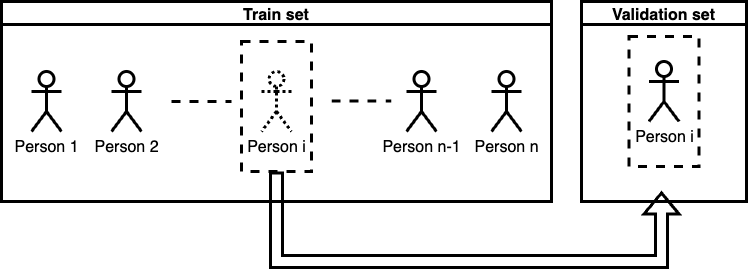
\includegraphics[width=0.75\linewidth]{Figure_4_LOSO cross-validation procedure.png}
    \caption{LOSO cross-validation procedure}
    \label{fig:enter-label}
\end{figure}

To rigorously assess the classification models' performance and generalization capabilities, two distinct validation strategies were employed: random splitting and leave-one-subject-out (LOSO) cross-validation. A detailed summary of these methodologies, including data split specifics, the number of iterations, and primary evaluation metrics, is presented in Table \ref{tab:cv_evaluation_setup}.

The random splitting technique was utilized to provide a baseline assessment of each model's ability to generalize to unseen data drawn from the same overall distribution. For this approach, the dataset was partitioned with a 70/30 random split, where 70\% of the data was allocated for training the models and the remaining 30\% was reserved for testing their performance.

To simulate a more challenging and realistic real-world scenario, particularly pertinent for user-independent applications such as advanced prosthetic control, LOSO cross-validation was implemented. This technique specifically evaluates a model's capacity to generalize to data from entirely new, previously unseen subjects. As visually conceptualized in Figure \ref{Eval_setup_metrics}, the LOSO procedure involves iteratively training the model on data from all subjects except for one, which is held out as the test set. This iterative process is repeated such that each subject serves as the test set precisely once. The final performance metrics are then calculated by averaging the results obtained across all these subject-specific iterations, yielding a robust estimate of the model's generalization capability to new individuals.

\begin{table}[!htbp]
\centering
\caption{Detailed Cross-Validation and Evaluation Setup}
\label{tab:cv_evaluation_setup}
\resizebox{\textwidth}{!}{%
\begin{tabular}{L{3cm} L{5cm} L{4cm} C{2cm} L{3.5cm} L{3cm}}
\toprule
\textbf{Validation Strategy} & \textbf{Description / Purpose} & \textbf{Data Split Details} & \textbf{No. of Iterations / Folds} & \textbf{Primary Performance Metrics Reported} & \textbf{Models Evaluated} \\
\midrule
\textbf{Random Splitting} & Assesses model generalization to unseen data from the same overall distribution; provides a baseline. & Dataset randomly split into training and testing sets. Ratio: 70\% for training, 30\% for testing. & 1 (single split per model run) & Accuracy, Weighted F1-score, Weighted Precision, Weighted Recall & XGBoost, Random Forest, SVM, CNN \\
\addlinespace
\textbf{LOSO Cross-Validation} & Evaluates model's ability to generalize to entirely new, unseen subjects, simulating real-world application to new users (user-independent evaluation). & Iteratively: N-1 subjects for training, 1 subject for testing (where N is total number of subjects). & N (10, as per 10 subjects in DB5) & Accuracy, Weighted F1-score (Mean $\pm$ SD reported across subjects) & XGBoost, Random Forest, SVM, CNN \\
\bottomrule
\end{tabular}%
}
\vspace{2mm}
\end{table}


% \subsubsection{Leave One Subject Out (LOSO)}

\subsection{Model analysis} \label{SHAP_sec}
SHAP, a game theory-based approach, quantifies the contribution of individual features to a model's prediction \cite{SHAP,TreeExplainer}. The SHAP value for a feature represents its average marginal contribution to the model's output across all possible feature combinations. Mathematically, the SHAP value for feature $i$ in instance $x$ is defined as:
($\phi_i(x)$) is defined as \begin{equation}
  \phi _i (x) = \sum _{S \subseteq F \setminus \{i\}} \frac{|S|!(|F|-|S|-1)!}{|F|!}[f_{S \cup \{i\}}(x_{S \cup \{i\}})-f_{S }(x_{S })]
\end{equation}  
 where :
 \begin{itemize}
   \item[] $x$: the observation input
   \item[] $F$: set of all features
   \item[] $f_S$: the trained model on the subset of features S
   
   \item[] $f_{S \cup \{i\}}$: the trained model on the subset of features 
S and \{i\}
  \item[] $x_S$: the restricted input of x given the subset of features S
  \item[] $x_{S \cup \{i\}}$: the restricted input of x given the subset of features 
S and \{i\}
 \end{itemize}


In the scope of this work, the SHAP score is presented as the average of the SHAP score by feature type or sensors. This will provide insights into the influence of each sEMG feature on the prediction of hand gestures as well as ranking the sensor influences on the driven model, furthering the understanding of the underlying mechanisms of movement detection in the system.

\subsection{Sensor quantity optimization}


This study introduced a sensor selection strategy aimed at optimizing the number of sensors required for effective performance. The sensor ranking, as determined in the preceding section (Section \ref{SHAP_sec}), serves as the basis for selecting the \textbf{i} most informative sensors. Subsequently, model training and validation were conducted using a random splitting validation scheme, the details of which are elaborated in Section \ref{Eval_setup_metrics}.

\section{Result and Discussion}
% \subsection{Baseline}
\subsection{Classification performance}
\begin{table}[h]
\centering
\caption{Hyperparameter settings for the classification models.}
\label{tab:hyperparameters}
\begin{tabular}{lll}
\hline
\textbf{Model} & \textbf{Parameter} & \textbf{Value/Setting} \\ \hline
\multirow{4}{*}{XGBoost} & Learning Rate & 0.XX \\
 & Max Depth & XX \\
 & N\_Estimators & XX \\
 & Objective & multi:softmax \\ \hline
\multirow{3}{*}{Random Forest} & N\_Estimators & XX \\
 & Criterion & Gini/Entropy \\
 & Min Samples Split & XX \\ \hline
\multirow{3}{*}{SVM} & Kernel & RBF/Linear \\
 & C (Regularization) & XX \\
 & Gamma & Scale/Auto \\ \hline
\multirow{4}{*}{CNN} & Optimizer & Adam/SGD \\
 & Learning Rate & 0.00XX \\
 & Batch Size & 32/64 \\
 & Epochs & XX \\ \hline
\end{tabular}
\end{table}

\begin{table}[!htbp]
\centering
\caption{The classification performance of models in random splitting scenarios (in percentage, higher is better)}
\label{tab:random_split_performance}
\resizebox{\textwidth}{!}{%
\begin{tabular}{l c c c c}
\toprule
\textbf{Metric (\%)} & \textbf{XGBoost} & \textbf{Random Forest} & \textbf{SVM} & \textbf{CNN} \\
\midrule
Accuracy            & 85 & 85 & 82 & 84 \\
\addlinespace % Adds a little extra visual separation between rows
Weighted F1-score   & 84 & 84 & 80 & 80 \\
\addlinespace
Weighted Precision  & 85 & 85 & 80 & 81 \\
\addlinespace
Weighted Recall     & 85 & 84 & 82 & 79 \\
\bottomrule
\end{tabular}%
} % End of resizebox
% \vspace{2mm} % This can be adjusted or removed if not needed
\end{table}

\begin{figure}[!ht]
\subfloat[Accuracy\label{pre_Acc_LOSO}]{
  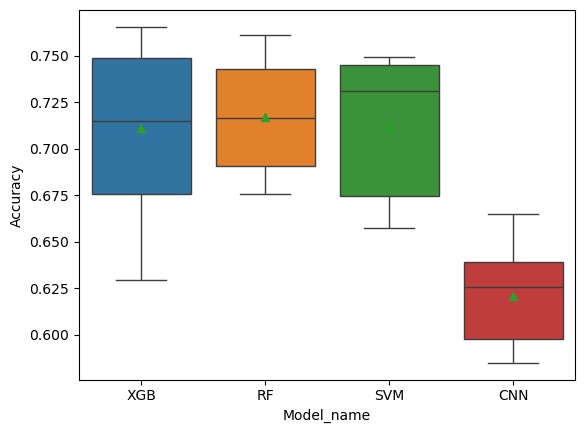
\includegraphics[width=0.45\linewidth]{Figure_5_a_Accuracy of ML models with LOSO validation .png}
}
% \caption{Random Forest}
% \label{fig_ShaplyRF}
% \end{subfigure}
% \hfill
% \begin{subfigure}[t]{0.24\textwidth}
\subfloat[Weighted F1  \label{pre_Weighted_LOSO}]{
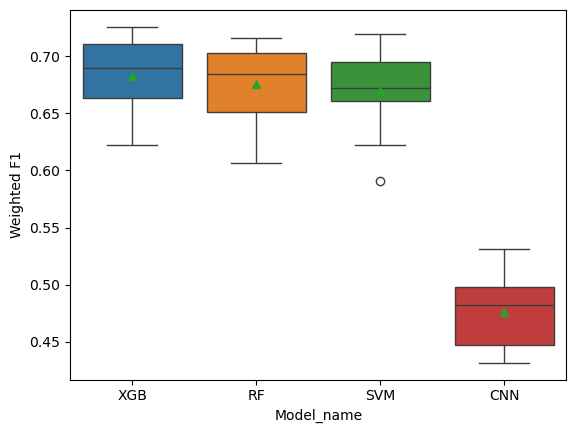
\includegraphics[width=0.45\linewidth]{Figure_5_b_Weighted F1 of ML models with LOSO validation .png}
}
% \caption{XGBoost model}
% \label{fig_ShaplyXG}
% \end{subfigure}
\caption{The (a) Accuracy, (b) Weighted F1 score of ML models with LOSO validation (higher is better)}
\label{pre LOSO}
\end{figure}

\begin{table}[!htbp]
\centering
\caption{Classification Performance of Models in Leave-One-Subject-Out (LOSO) Cross-Validation}
\label{tab:loso_performance_summary}
\resizebox{\textwidth}{!}{%
\begin{tabular}{l c c c c}
\toprule
\textbf{Metric (Mean \% $\pm$ SD)} & \textbf{XGBoost} & \textbf{Random Forest} & \textbf{SVM} & \textbf{CNN} \\
\midrule
Accuracy & $71 \pm 4$ & $71 \pm 4$ & $73 \pm 3$ & \textit{$\sim 61.5 \pm \text{5}$} \\
\addlinespace % Adds a little extra visual separation
Weighted F1-score & $68 \pm 4$ & $67 \pm 4$ & $65 \pm 4$ & \textit{$\sim 48 \pm \text{6}$} \\

\bottomrule
\end{tabular}%
} % End of resizebox
\vspace{2mm}
\end{table}


In the context of random splitting, as illustrated in Table \ref{tab:random_split_performance}, the XGB and RF models exhibited a surpassed performance in recognizing finger positions, achieving an accuracy of approximately 85\% in comparison with SVM and CNN models. Regarding the weighted F1 score, the XGB and RF models also outperformed their counterparts, reaching values as high as 84\%, reflecting a 4\% improvement over the SVM and CNN models.

In LOSO validation, the XGB, RF, and SVM models demonstrated comparable results, achieving approximately 71 ± 4\% accuracy and a weighted F1 score of 68 ± 4\% (see Figure \ref{pre LOSO}). Interestingly, the CNN model, despite its competitive performance in the random splitting phase, exhibited a noticeable decline in accuracy during LOSO validation. The reduction in performance under LOSO validation should not be attributed exclusively to algorithmic overfitting. It also reflects substantial biological and measurement variability across individuals, including muscle architecture, subcutaneous tissue, skin–electrode impedance, armband orientation, and subject-specific motor-unit recruitment. Thus, two individuals performing the same finger movement may generate different multichannel activation distributions. The LOSO results therefore provide a more stringent assessment of whether the classifier captures movement-related neuromuscular structure that generalizes beyond subject-specific electrode–muscle relationships.

In summary, the XGB and RF models consistently delivered the most robust performance across evaluation scenarios, achieving an accuracy of up to 85\% in the random splitting phase and approximately 71 ± 4\% in LOSO validation.

\subsection{Feature analysis}

\begin{figure}[!ht]
\subfloat[XGBoost\label{FI_xgb}]{
    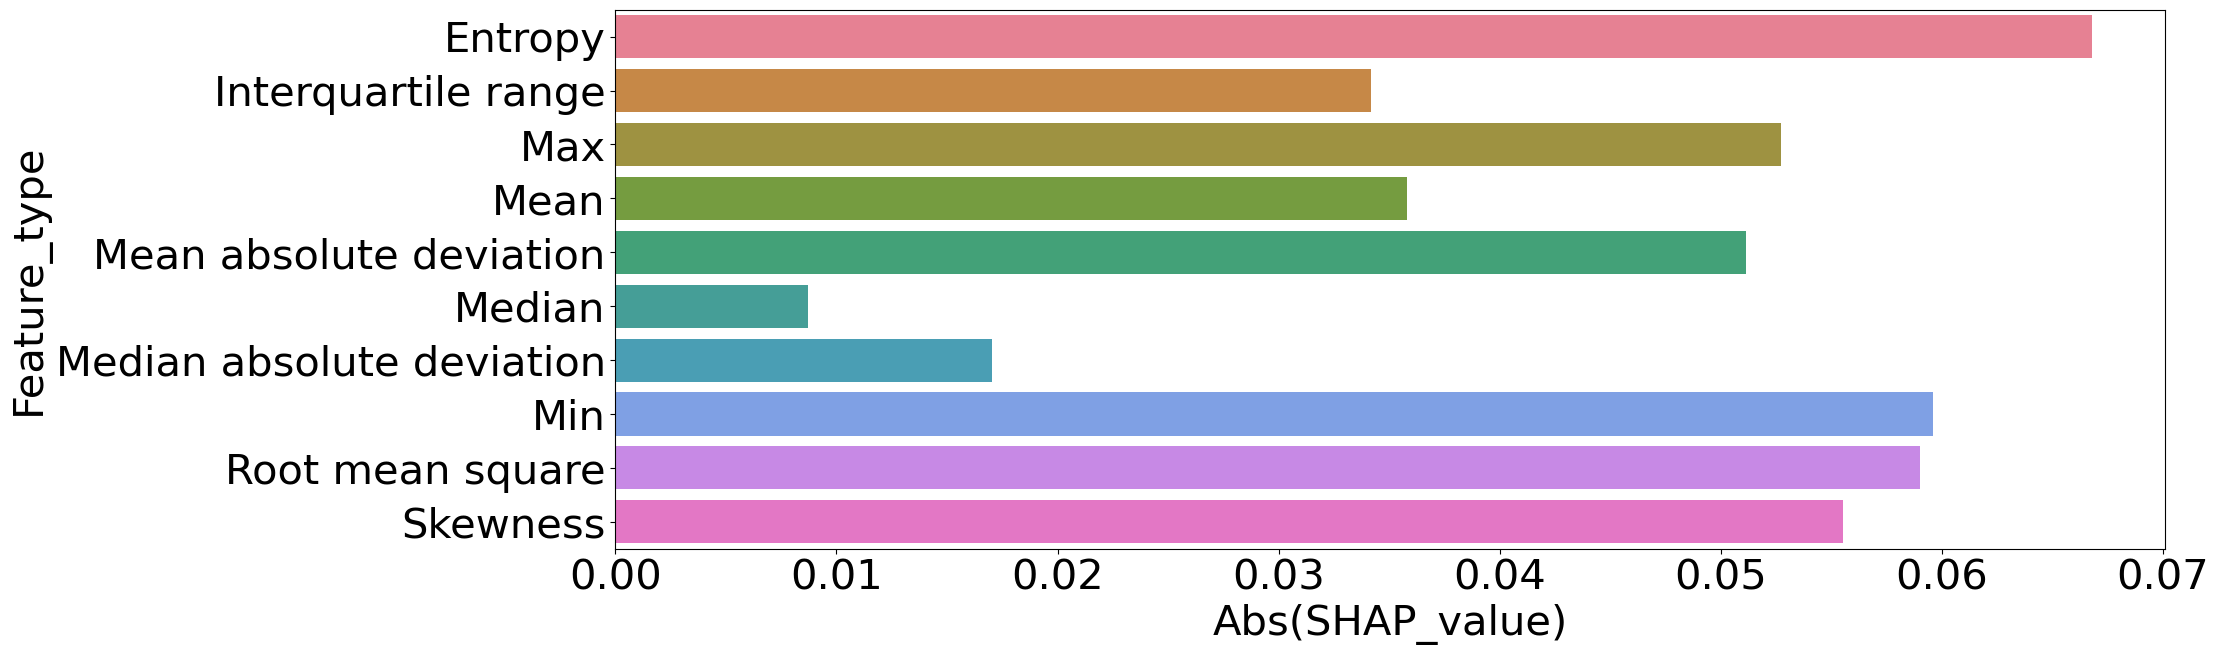
\includegraphics[width=0.45\linewidth,height=0.2\linewidth]{Figure_6_a_FI_by_features_xgb.png}
}
% \caption{Random Forest}
% \label{fig_ShaplyRF}
% \end{subfigure}
% \hfill
% \begin{subfigure}[t]{0.24\textwidth}
\subfloat[Random Forest  \label{FI_rf}]{
    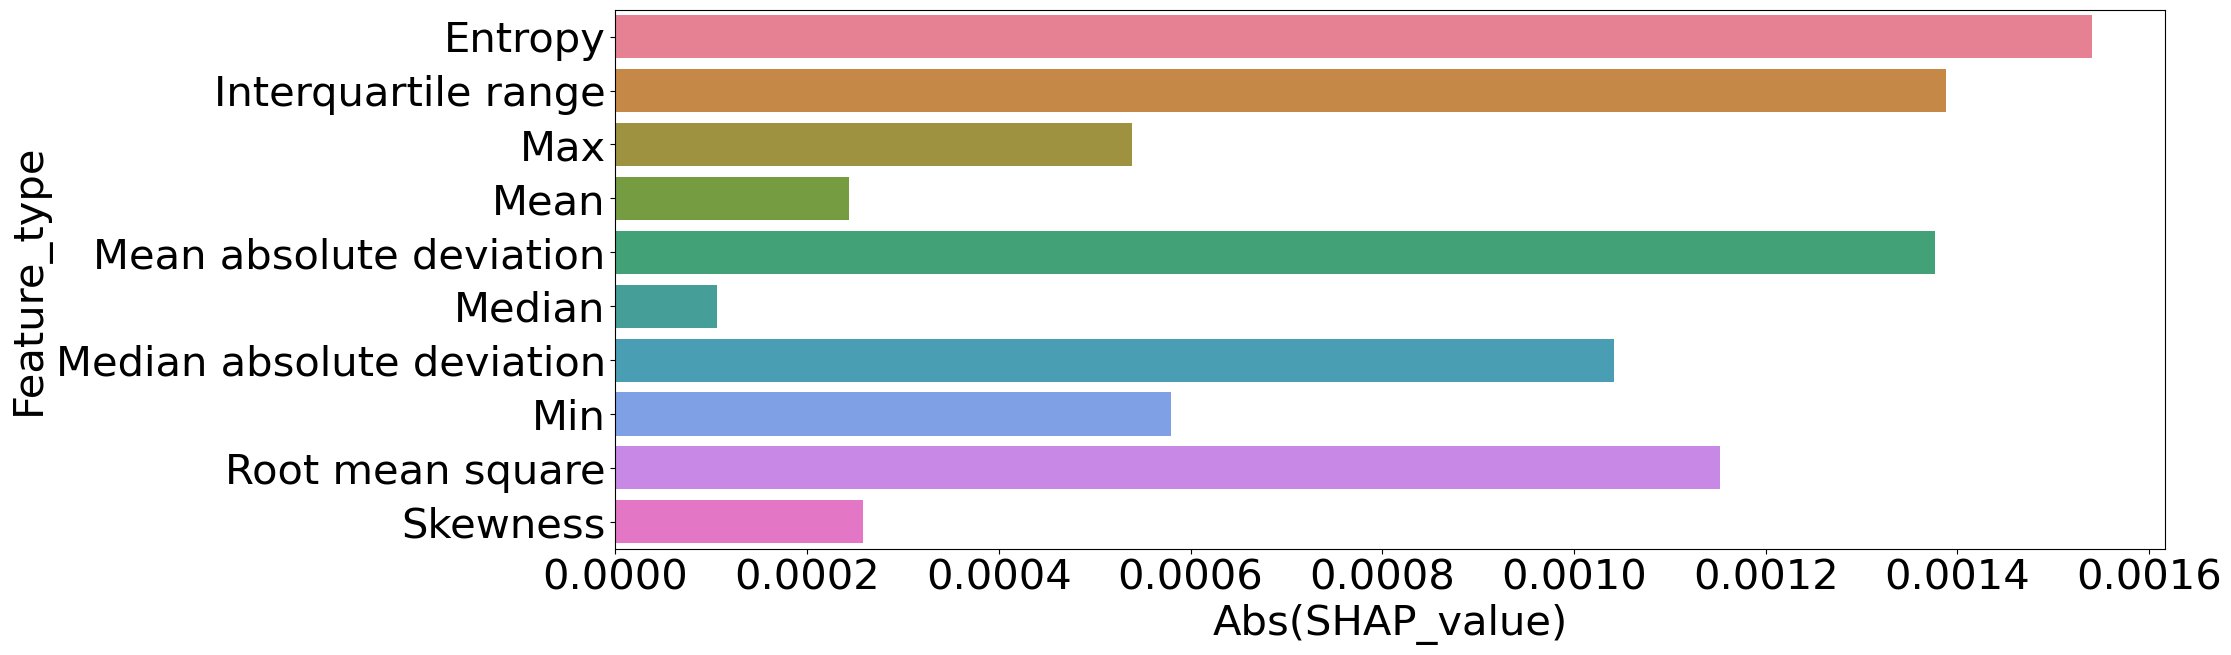
\includegraphics[width=0.45\linewidth,height=0.2\linewidth]{Figure_6_b_FI_by_Features_rf.png}
}
% \caption{XGBoost model}
% \label{fig_ShaplyXG}
% \end{subfigure}
\caption{Feature contributions in XGBoost (a) and Random Forest (b) models (SHAP Analysis) using random splitting test on 12 finger position classification}
\label{featIM_feat}
\end{figure}


\begin{figure}[!ht]
\subfloat[XGBoost\label{FI_xgb2}]{
    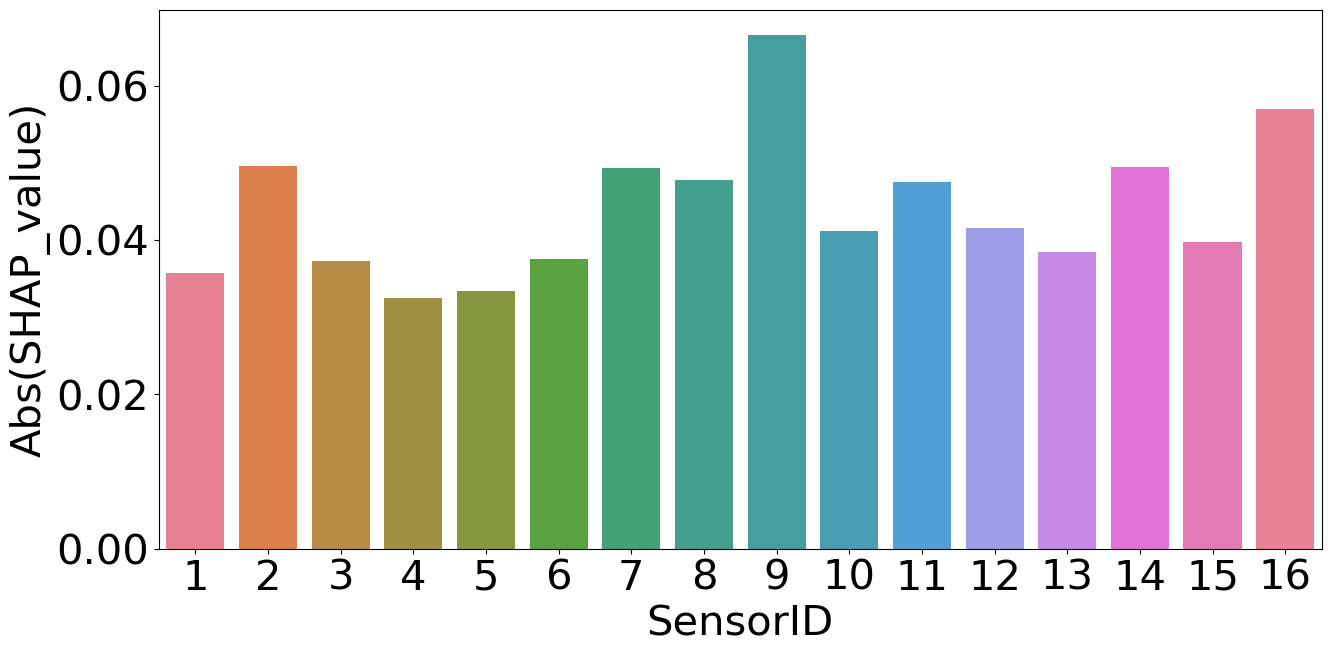
\includegraphics[width=0.45\linewidth]{Figure_7_a_FI_by_sensors_xgb.png}
}
% \caption{Random Forest}
% \label{fig_ShaplyRF}
% \end{subfigure}
% \hfill
% \begin{subfigure}[t]{0.24\textwidth}
\subfloat[Random Forest  \label{FI_rf2}]{
    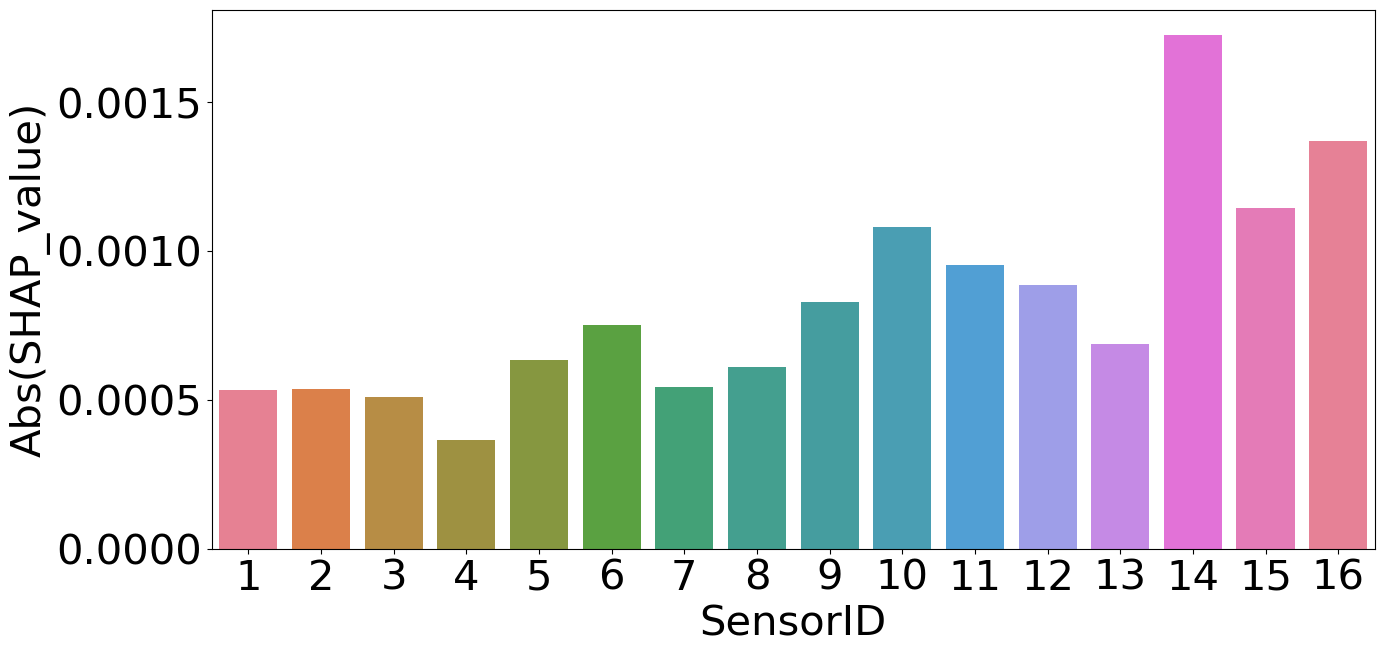
\includegraphics[width=0.45\linewidth]{Figure_7_b_FI_by_sensors_rf.png}
}

\caption{Sensor contributions in XGBoost (a) and Random Forest (b) models (SHAP Analysis) using random splitting test on 12 finger positions classification}
\label{featIM_sen}
\end{figure}

\begin{table}[!htbp]
\centering
\caption{Mean Absolute SHAP Values for time-domain features in XGBoost and random forest models (random split)}
\label{tab:feature_shap_contributions}
% \resizebox{\textwidth}{!}{%
\begin{tabular}{L{0.3\textwidth} L{0.3\textwidth} L{0.3\textwidth}}
\toprule
\textbf{Feature Type} & \textbf{Mean Absolute SHAP Value (XGBoost)} & \textbf{Mean Absolute SHAP Value (Random Forest)} \\
\midrule
Entropy                     & \textit{$\sim 0.066$} & \textit{$\sim 0.00160$} \\
\addlinespace
Root Mean Square (RMS)      & \textit{$\sim 0.060$} & \textit{$\sim 0.00115$} \\
\addlinespace
Minimum (Min)               & \textit{$\sim 0.061$} & \textit{$\sim 0.00055$} \\
\addlinespace
Interquartile Range (IQR)   & \textit{$\sim 0.035$} & \textit{$\sim 0.00125$} \\
\addlinespace
Mean Absolute Deviation     & \textit{$\sim 0.050$} & \textit{$\sim 0.00140$} \\
\addlinespace
Maximum (Max)               & \textit{$\sim 0.052$} & \textit{$\sim 0.00050$} \\
\addlinespace
Skewness                    & \textit{$\sim 0.055$} & \textit{$\sim 0.00025$} \\
\addlinespace
Mean                        & \textit{$\sim 0.035$} & \textit{$\sim 0.00020$} \\
\addlinespace
Median                      & \textit{$\sim 0.010$} & \textit{$\sim 0.00015$} \\
\addlinespace
Median Absolute Deviation   & \textit{$\sim 0.020$} & \textit{$\sim 0.00005$} \\
\bottomrule
\end{tabular}%
% } % End of resizebox
\vspace{2mm}
\end{table}

\begin{table}[!htbp]
\centering
\caption{Sensor contribution ranking based on mean absolute SHAP values for XGBoost and random forest models (random split)}
\label{tab:sensor_shap_ranking}
% \resizebox{\textwidth}{!}{
\begin{tabular}{L{0.08\textwidth} L{0.16\textwidth} L{0.25\textwidth} L{0.14\textwidth} L{0.2\textwidth}}
\toprule
\textbf{Rank} & \textbf{Sensor ID (XGB)} & \textbf{Mean Abs SHAP (XGB)} & \textbf{Sensor ID (RF)} & \textbf{Mean Abs SHAP (RF)} \\
\midrule
1  & 9  & \textit{$\sim 0.068$} & 14 & \textit{$\sim 0.00170$} \\
\addlinespace
2  & 16 & \textit{$\sim 0.058$} & 16 & \textit{$\sim 0.00150$} \\
\addlinespace
3  & 7  & \textit{$\sim 0.049$} & 11 & \textit{$\sim 0.00110$} \\
\addlinespace
4  & 10 & \textit{$\sim 0.048$} & 10 & \textit{$\sim 0.00100$} \\
\addlinespace
5  & 14 & \textit{$\sim 0.048$} & 9  & \textit{$\sim 0.00090$} \\
\addlinespace

\bottomrule
\end{tabular}%
% } % End of resizebox
% \vspace{2mm}
\end{table}


The feature importance analysis unveiled that entropy emerged as the most influential feature in both the XGB and RF models with the summary in Table \ref{tab:feature_shap_contributions}. This is evident from the mean SHAPley values: 0.066 for XGB and 0.0016 for RF (Figures \ref{FI_xgb} and \ref{FI_rf}). Entropy's significant contribution can be attributed to its capacity to capture the dynamic and stochastic nature of sEMG signals during movement.

In addition to entropy, simple time-domain features such as minimum, maximum, IQR, and RMS were found to be highly informative. These features, which are relatively straightforward to compute, demonstrated a strong correlation with finger position classification. This finding reinforces the notion that simple statistical features can be highly effective in sEMG-based systems.

From a physiological perspective, the importance of RMS and amplitude-distribution features is consistent with their sensitivity to the aggregate electrical activity generated by recruited motor units within each analysis window. RMS provides an amplitude-related measure of the recorded sEMG signal, whereas entropy characterizes the irregularity and distributional complexity of the signal. During finger movement, changes in motor-unit recruitment, discharge timing, and the relative contribution of synergistic muscles alter both the amplitude and complexity of the recorded waveform. Accordingly, the high attribution assigned to entropy and RMS suggests that the classifiers used complementary information concerning the intensity and temporal organization of neuromuscular activation. These features should not, however, be interpreted as direct measurements of muscle force or individual motor-unit behavior, because each channel contains a volume-conducted mixture of multiple physiological sources.

Regarding sensor importance, a detailed quantitative ranking based on mean absolute SHAP values for both the XGBoost and Random Forest models is presented in Table \ref{tab:sensor_shap_ranking}. As visually illustrated in Figures \ref{FI_xgb2} (for XGBoost) and \ref{FI_rf2} (for Random Forest), and further detailed in Table \ref{tab:sensor_shap_ranking}, sensor 9 demonstrated the most significant impact on XGBoost model decisions, while sensor 14 exhibited a high influence on the Random Forest model's performance. Notably, the analysis consistently highlighted sensors 9, 10, 11, 14, and 16 as having high SHAPley values across these models, underscoring their critical role in the accurate recognition of finger positions.

% \begin{figure}
%     \centering
%     \includegraphics[width=1\linewidth]{GradCam_Output0.png}
%     \caption{Visualization of Grad-CAM for the output 0}
%     \label{grad_0}
% \end{figure}

% \begin{figure}
%     \centering
%     \includegraphics[width=1\linewidth]{GradCam_Output1.png}
%     \caption{Visualization of Grad-CAM for the output 1}
%     \label{grad_1}
% \end{figure}
\begin{figure}[!ht]
    \centering
    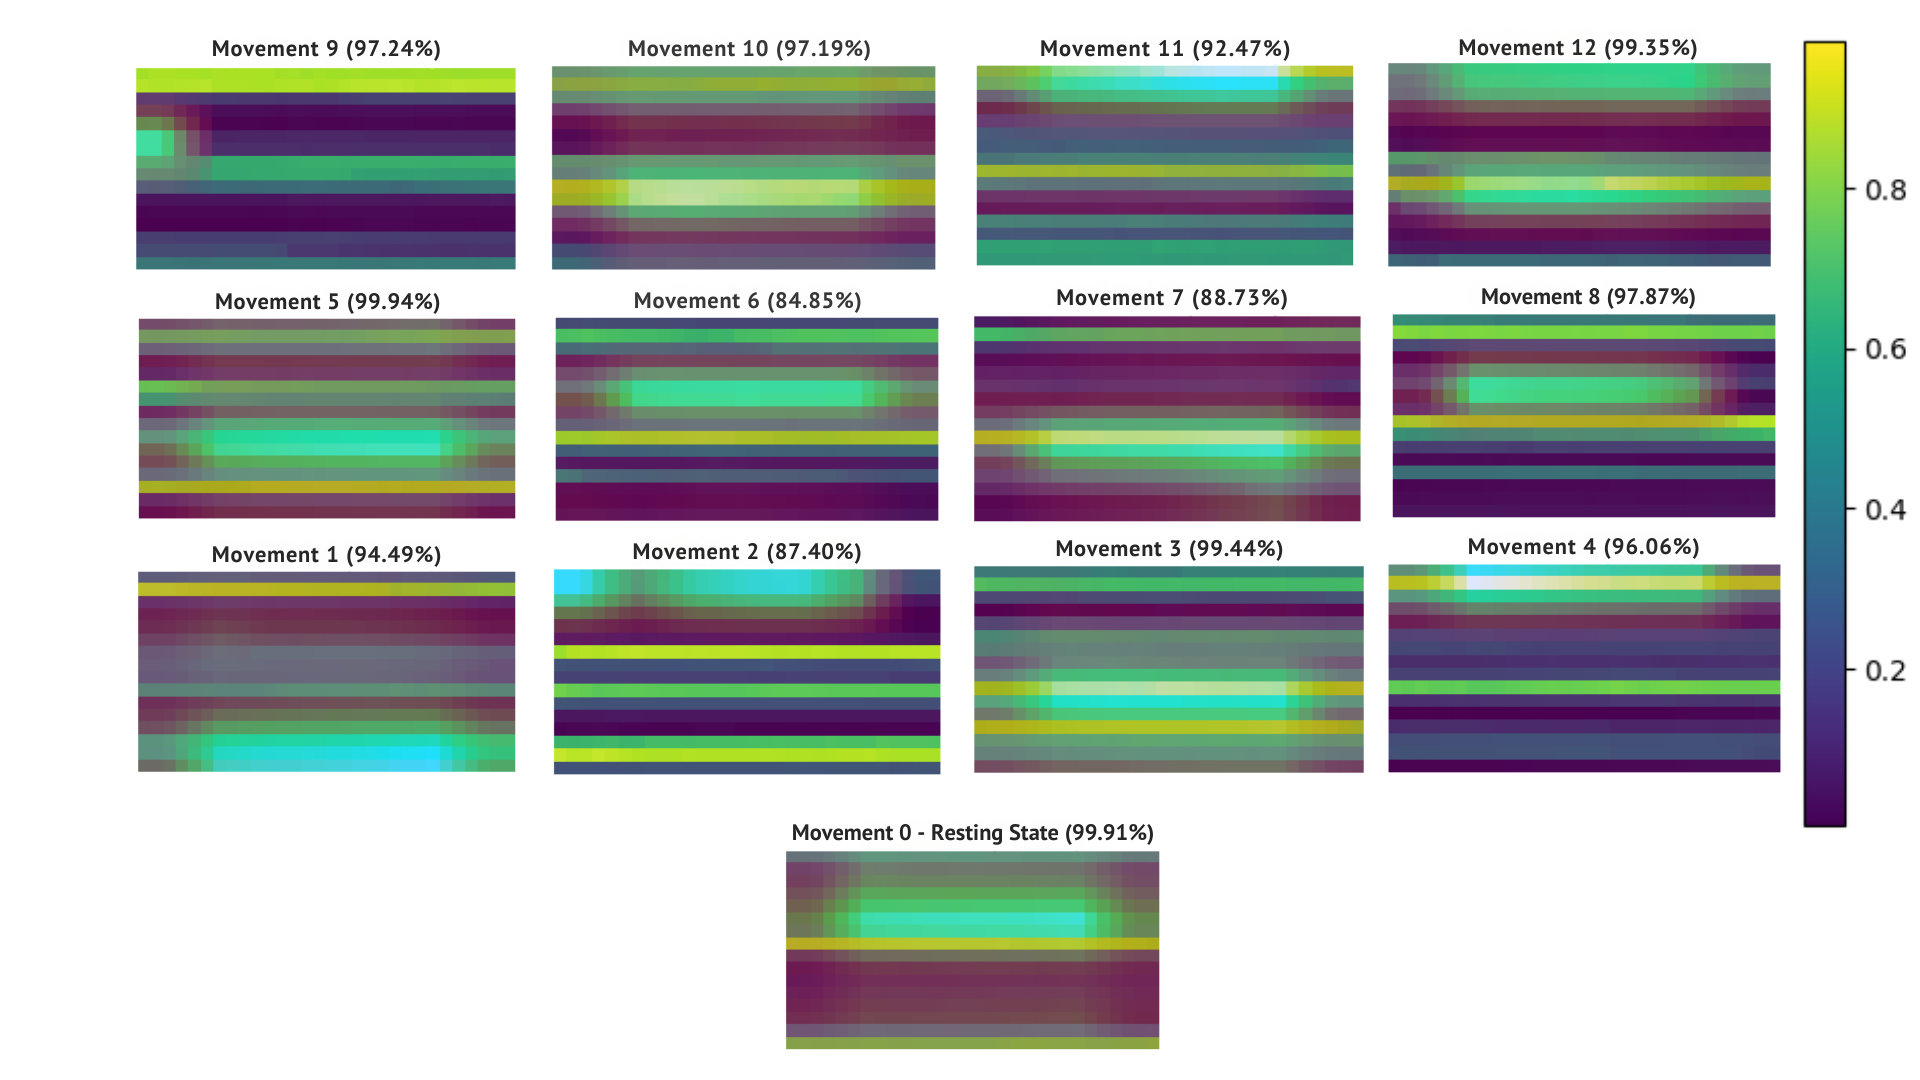
\includegraphics[width=1\linewidth]{Figure_8_Class-Specific Grad-CAM heatmaps for 13 outputs.png}
    \caption{Class-Specific Grad-CAM heatmaps for 13 outputs in sEMG-Based fingers recognition. The vertical axis of each heatmap corresponds to sensors arranged sequentially from 0 to 16, while the horizontal axis represents data points segmented into 100 sample windows, equivalent to a temporal resolution of 500 ms.}
    \label{grad_1}
\end{figure}

\begin{table}[!htbp]
\centering
\caption{Structured Summary of CNN Grad-CAM Observations and Interpretations for Finger Movements}
\label{tab:gradcam_summary_revised}
\resizebox{\textwidth}{!}{%
\begin{tabular}{L{1.2cm} L{2cm} C{2cm} L{6cm} L{6cm} L{6cm}}
\toprule
\textbf{Mov. No.} & \textbf{Movement Name} & \textbf{Predicted Prob.(\%)} & \textbf{ Key Activated Sensor Regions/Channels} & \textbf{Implied Neuromuscular Dynamics / Anatomical Muscle Groups} & \textbf{Noteworthy Observation} \\
\midrule

0 & Resting State & 99.91 & Diffuse, low-intensity activation across most channels; a slightly more prominent central horizontal band. & Baseline muscle tone; minimal distinct activation. & High confidence (99.91\%), clear distinction from active movements. \\
\addlinespace

1 & Index Flexion & 94.49 & Strong, fairly symmetrical activation in upper-middle horizontal bands, prominent across several central channels. & Flexor Digitorum Superficialis (FDS), Flexor Digitorum Profundus (FDP). & Exhibits bilateral symmetry, indicating balanced contributions from EMG armband sensors. Aligns with anterior compartment flexor muscles. \\
\addlinespace

2 & Index Extension & 87.40 & Symmetrical activation, more focused in the central horizontal bands, distinct from flexion pattern. & Extensor Digitorum Communis (EDC). & Also shows bilateral symmetry. Aligns with posterior compartment extensor muscles. Complementary roles effectively captured. \\
\addlinespace

3 & Middle Flexion & 99.44 & Strong, symmetrical activation, similar to index flexion but potentially engaging slightly different or broader central channel groups. & FDS, FDP (tendons for middle finger). & Similar symmetry observed as for index finger movements. Reflects compartmentalized but overlapping muscle activity. \\
\addlinespace

4 & Middle Extension & 96.06 & Symmetrical activation in central horizontal bands, pattern distinct from middle flexion. & EDC (tendons for middle finger). & Similar symmetry observed, consistent with coordinated extension. \\
\addlinespace

5 & Ring Flexion & 99.94 & Strong, symmetrical activation, concentrated in central horizontal bands, possibly overlapping with index/middle flexion regions. & FDS, FDP (tendons for ring finger). & Similar symmetry observed. \\
\addlinespace

6 & Ring Extension & 84.85 & Symmetrical activation, somewhat more diffuse than other extensions but still focused in central horizontal bands. & EDC (tendons for ring finger). & Similar symmetry observed. \\
\addlinespace

7 & Little Finger Flexion & 88.75 & Symmetrical activation, prominent in central horizontal bands, possibly slightly lower or more lateral than other finger flexions. & FDS, FDP (tendons for little finger). & Similar symmetry observed. \\
\addlinespace

8 & Little Finger Extension & 97.87 & Symmetrical activation in central horizontal bands, pattern distinct from little finger flexion. & EDC (tendons for little finger). & Similar symmetry observed. \\
\addlinespace

9 & Thumb Adduction & 97.24 & Activation more concentrated, possibly less broad horizontally than finger movements, prominent in specific channel groups related to thumb adductor muscles. & Adductor Pollicis, potentially Flexor Pollicis Brevis. & Activation maps reveal spatial relevance reflecting neuromuscular dynamics. \\
\addlinespace

10 & Thumb Abduction & 97.19 & Distinct activation pattern, likely engaging sensors near the thumb's base and radial side of the forearm. & Abductor Pollicis Longus, Abductor Pollicis Brevis. & Spatial correspondence between sensor activations and flexion-extension cycles highlights importance of precise sensor placement. \\
\addlinespace

11 & Thumb Flexion & 92.47 & Focused activation related to thumb flexor muscles, potentially in lower or more central sensor bands compared to finger flexions. & Flexor Pollicis Longus, Flexor Pollicis Brevis. & Consistent identification of a central "activation band" across visualizations. \\
\addlinespace

12 & Thumb Extension & 99.35 & Clear activation pattern for thumb extension, likely engaging sensors on the dorsal/radial aspect of the forearm. & Extensor Pollicis Longus, Extensor Pollicis Brevis. & Grad-CAM visualizations offered compelling evidence of CNN's ability to identify and prioritize critical features. \\
\bottomrule
\end{tabular}%
}
\end{table}




%To comprehensively evaluate the feature recognition capabilities of the CNN, we use Gradient-weighted Grad-CAM visualizations, as illustrated in Figure \ref{grad_1}. Grad-CAM offers an interpretable representation of the network's focus by highlighting the input regions that contribute most significantly to its classification decisions. 

The Grad-CAM results in Figure \ref{grad_1} demonstrate the model's robust ability to classify 13 distinct finger gestures, including flexion and extension movements of the fingers and thumb, with high confidence. Interestingly, while visual inspection of the CNN input images did not detect significant differences across EMG channels, the Grad-CAM maps exhibited movement-dependent differences between finger-flexion, finger-extension, and thumb-related classes. Such differentiation is physiologically plausible because flexion and extension are generated by functionally distinct but spatially overlapping forearm muscle compartments. The predicted movements, displayed alongside their respective probabilities, indicate a classification reliability ranging from 80\% to 99\%, underscoring the strength of CNN in distinguishing subtle variations in EMG signals. This result highlighted the ability of Grad-CAM to uncover subtle yet crucial features that are not immediately apparent from the raw input, providing a deeper understanding of the CNN's decision-making process.

The activation maps reveal the spatial relevance of individual sensors to specific movements, reflecting the neuromuscular dynamics underlying these gestures. For index finger flexion and extension (Movements 1 and 2), the Grad-CAM visualizations exhibit spatially distributed activation across the two sEMG armbands. This pattern aligns with the anatomical structure of the forearm, where flexor muscles, such as the flexor digitorum superficialis (FDS) and flexor digitorum profundus (FDP), are located in the anterior compartment, while extensor muscles, including the extensor digitorum communis (EDC), are situated in the posterior compartment \cite{Kikuchi}. The FDS and FDP contribute to flexion of multiple digits, whereas EDC and associated digit-specific extensors contribute to extension. Their shared tendons, mechanical coupling, and common neural inputs also limit complete independence among the fingers. Therefore, the relevant physiological signature is not expected to be a single isolated channel for each digit; rather, it should appear as a distributed pattern whose relative weighting changes across movement classes.

Similar symmetry is observed for movements of the middle (Movements 3 and 4), ring (Movements 5 and 6), and little fingers (Movements 7 and 8) (Figure \ref{grad_1}) . These findings reflect compartmentalized but overlapping muscle activity in the forearm, where FDS and FDP provide separate tendons for individual fingers, while interconnected tendons of the EDC contribute to coordinated extension across multiple digits \cite{Leijnse}.

The spatial correspondence between sensor activations and flexion-extension cycles highlights the importance of precise sensor placement to accurately capture localized muscle activations. Furthermore, this symmetry reinforces the physiological basis for coordinated muscle activity, where agonist and antagonist muscle groups work together to minimize energy expenditure and enhance movement precision, resulting in consistent and balanced EMG signals across the forearm \cite{Enoka}.

By integrating these physiological insights, the Grad-CAM results validate the CNN's ability to map sensor activations to underlying neuromuscular dynamics. This connection between anatomy and AI-driven analysis emphasizes the robustness of the model in interpreting complex hand movements using sEMG signals. The hierarchical feature extraction process of CNNs, where initial convolutional layers capture fine-grained spatial and temporal patterns refined by deeper layers, likely contributes to this ability \cite{liu}. This robustness is critical for applications in prosthetic control, rehabilitation, and gesture recognition, where detecting minimal neuromuscular changes is essential for accurate system responses \cite{putcha}. Optimizing the signal preprocessing pipeline to retain low-amplitude components further enhances the model's capability to utilize these signals in decision-making.

%Interestingly, the Grad-CAM visualizations reveal that the CNN effectively leverages low-intensity sEMG signals for static hand postures or movements with minimal muscle activation. The muted but discernible activation regions in the heatmaps highlight the sensitivity of the network to subtle variations in these signals, reflecting baseline neuromuscular activity or minor fluctuations in muscle recruitment. This capability is particularly valuable for fine-grained movement classification and aligns with previous findings in myoelectric signal analysis, where low-amplitude sEMG signals have been shown to contain crucial information for distinguishing between static and dynamic states or recognizing subtle gestures \cite{Tchantchane, ghaffar}.


Another notable observation is the consistent identification of a central "activation band" across visualizations (Figure \ref{grad_1}). This feature indicates the CNN's capacity to prioritize task-relevant features from sEMG input data \cite{stuart2024adaptable}. Additionally, the relatively small variations in confidence levels across movements point to areas for optimization, such as resolving feature overlaps or refining ambiguous patterns.

In short, Grad-CAM visualizations offered compelling evidence of CNN's ability to identify and prioritize critical features for accurate gesture classification. These visualizations illuminated the spatial and temporal interplay of sensor activations in capturing flexion-extension patterns for individual fingers. The explainability provided by Grad-CAM not only validated model performance but also informed improvements in sensor placement and preprocessing. The insights derived from these visualizations play an integral role in optimizing the sensor configuration pipeline (see Section \ref{proposed pipeline}), ultimately improving the efficiency and accuracy of the system.

\subsection{Sensor selection}\label{proposed pipeline}
% \begin{figure}[!ht]
%     \centering
%     \includegraphics[width=0.75\linewidth]{Propose_pipeline _acc.png}
%     \caption{The Line chart of number of sensors and accuracy in propose pipeline}

%     \label{Propose_pipeline_acc}
% \end{figure}
% \begin{figure}[!ht]
%         \centering
%         \includegraphics[width=0.75\linewidth]{Propose_pipeline _F1.png}
%         \caption{The Line chart of number of sensors and weighted F1 in propose pipeline}
%         \label{Propose_pipeline_f1}
% \end{figure}



\begin{figure}[!ht]
\subfloat[Accuracy\label{Propose_pipeline_acc}]{
  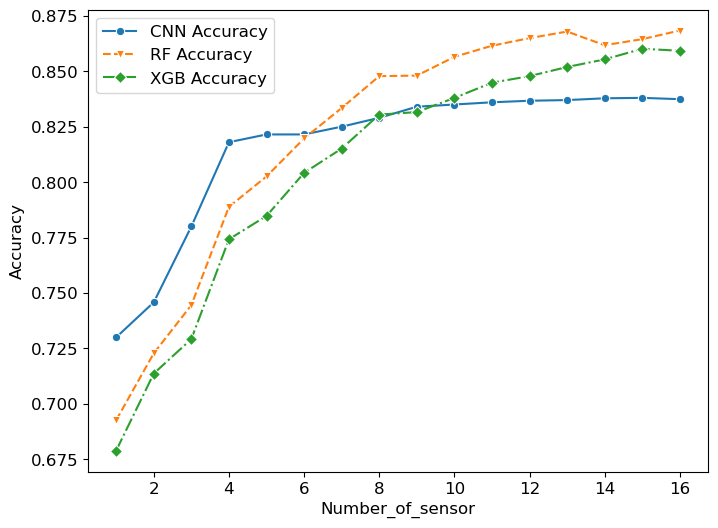
\includegraphics[width=0.45\linewidth]{Figure_9_a_Propose_pipeline _acc.png}
}
% \caption{Random Forest}
% \label{fig_ShaplyRF}
% \end{subfigure}
% \hfill
% \begin{subfigure}[t]{0.24\textwidth}
\subfloat[Weighted F1  \label{Propose_pipeline_f1}]{
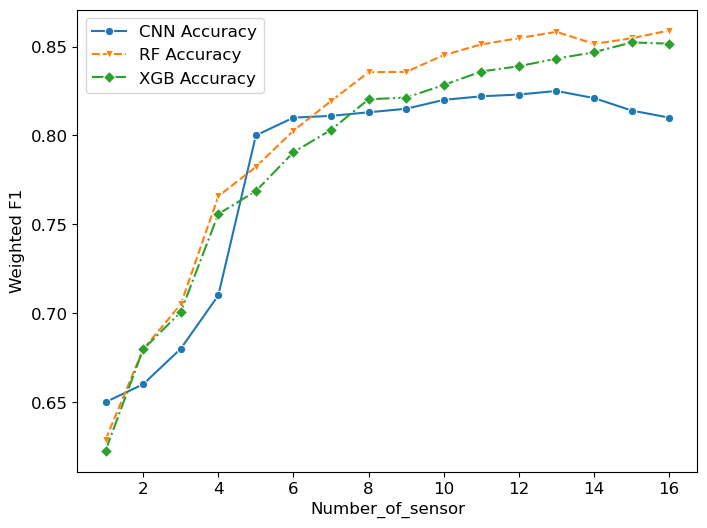
\includegraphics[width=0.45\linewidth]{Figure_9_b_Propose_pipeline _F1.png}
}
% \caption{XGBoost model}
% \label{fig_ShaplyXG}
% \end{subfigure}
\caption{ Impact of sensor quantity on model performance in the  (a) accuracy, (b) weighted F1 score in the XAI-integrated finger position classification models}
\label{Propose_pipeline_SS}
\end{figure}
% By utilizing the sensor importance (see Figure \ref{featIM_sen}) to our propose pipeline (see Figure \ref{method_fc})

The XAI-integrated models demonstrated a positive correlation between the number of sensors employed and the resultant model performance, as depicted in Figures \ref{Propose_pipeline_acc} and \ref{Propose_pipeline_f1}. Initially, with a single optimal sensor, both XGB and RF models exhibited comparable performance, achieving accuracies of approximately 67\% and weighted F1 scores of approximately 61\%.

Subsequent integration of additional sensors, however, yielded substantial performance improvements. Notably, in the configuration utilizing the eight most informative sensors, the overall accuracy increased to approximately 84\%, and the weighted F1 score reached over 80\%. Beyond this point, further expansion of the sensor array resulted in diminishing returns, contributing only an additional 3\% gain in accuracy and a 5\% increase in the weighted F1 score.

In comparison, the CNN model exhibited a robust initial weighted F1 score of approximately 75\% with a single sensor, which rapidly improved to 81\% with four sensors, followed by a performance plateau. Conversely, the CNN model's accuracy, while starting at 65\% with a single sensor, experienced a significant increase to 80\% with the inclusion of five sensors, beyond which no further improvement was observed.

These findings suggest that for practical implementation in real-world finger-recognition applications, a configuration employing 5 to 10 sensors offers a pragmatic balance between complexity and performance. Nonetheless, to achieve maximal performance, the incorporation of a more extensive sensor array and the extraction of more complex features are recommended.

This result highlighted the potential for optimizing the number of sEMG sensors required for accurate gesture recognition. By leveraging XAI techniques, the research identifies the most influential sensors and demonstrates that a system with 5 to 10 sensors can achieve performance comparable to setups with 16 sensors. This finding has significant implications for the practical deployment of prosthetic devices, as reducing the number of sensors can lower costs, improve comfort, and simplify the setup process for users.However, the study also raises questions about the trade-offs between sensor reduction and performance. While the results suggest that a reduced number of sensors can still achieve high accuracy, further research is needed to explore how this reduction impacts the system's robustness in real-world scenarios, such as during prolonged use or under varying muscle fatigue conditions. Additionally, the placement of sensors may need to be reconsidered to ensure that the most critical muscle signals are captured effectively.

\section{Conclusion}

In this work, XAI-integrated classification models were developed to detect the hand position with high accuracy while minimizing the required input. By incorporating XAI methods like SHAP and Grad-CAM, the interpretability of machine learning models was significantly improved, and valuable insights into the factors influencing model decisions were gained. The CNN model achieved a classification accuracy reaching up to 85\% for finger position recognition and 72\% for person-independent recognition when utilizing all 16 sensors. Additionally, the optimization of sEMG sensors configuration using 5 to 10 sensors could achieve comparable performance, with an accuracy of 84\% and a weighted F1 score of 80\%, making it a practical solution for real-world applications. By leveraging XAI, the proposed framework not only improves the accuracy and interpretability of gesture recognition but also lays the groundwork for more personalized and user-centric prosthetic devices.

% Our study underscores the importance of simple time-domain features, particularly entropy, in capturing the dynamic nature of finger movements. This suggests that computationally efficient features can be highly effective in sEMG-based systems, paving the way for more cost-effective and user-friendly prosthetic devices. Furthermore, the use of XAI techniques allows for a deeper understanding of individual sensor contributions and feature impacts, enabling the optimization of sensor configurations and enhancing overall system efficiency.

% Despite these promising outcomes, several areas for future improvement remain. The generalizability of our framework across diverse populations and real-world conditions is a critical challenge. Factors such as inter-subject variability, muscle fatigue, and electrode placement differences need to be addressed to ensure robust performance in clinical settings. Additionally, while our study demonstrates the potential of XAI in enhancing model transparency, further work is needed to evaluate how these explanations are communicated to end-users, especially those without technical expertise. Developing user-friendly interfaces and integrating feedback from clinicians and patients will be crucial for building trust and facilitating the adoption of XAI-enhanced prosthetic systems.

% In summary, this study represents a significant advancement in the development of sEMG-based prosthetic control systems. By leveraging XAI, the proposed framework not only improves the accuracy and interpretability of gesture recognition but also lays the groundwork for more personalized and user-centric prosthetic devices. Future research should focus on addressing the identified limitations, exploring real-time applications, and extending the framework to other types of prosthetic control. With continued advancements in AI and rehabilitation robotics, this work contributes to a future where individuals with limb differences can regain greater autonomy and improve their quality of life through intuitive and reliable prosthetic technologies.

\section*{Acknowledgements}

\bibliographystyle{elsarticle-num} 


\bibliography{bib}

%% else use the following coding to input the bibitems directly in the
%% TeX file.

% \begin{thebibliography}{00}

% %% \bibitem{label}
% %% Text of bibliographic item

% \bibitem{}

% \end{thebibliography}
\end{document}
\endinput
%%
%% End of file `elsarticle-template-num.tex'.
